\documentclass[%
pdf,
%nocolorBG,
colorBG,
slideColor,
%slideBW,
%draft,
%frames
%azure
%contemporain
%nuancegris
%troispoints
%lignesbleues
%darkblue
%alienglow
%autumn
]{prosper}
\usepackage{pifont, amsmath, multicol}
%\usepackage{floatflt, wrapfig,subfigure}
%\usepackage{wrapfig}
%\usepackage{floatflt}
\usepackage{color}
\usepackage{epsfig}
\usepackage{pifont}
%\usepackage[francais]{babel}
\usepackage[T1]{fontenc}
\usepackage[latin1]{inputenc}
%\def«{\og\ignorespaces}%
%\def»{{\fg}}%
\newcommand{\spacer}{\rule[-3mm]{0mm}{8mm}}

\newcommand{\RR}{\ensuremath{\mathbb{R}}}
\newcommand{\NN}{\ensuremath{\mathbb{N}}}
\newcommand{\QQ}{\ensuremath{\mathbb{Q}}}
\newcommand{\CC}{\ensuremath{\mathbb{C}}}
\newcommand{\ZZ}{\ensuremath{\mathbb{Z}}}
\newcommand{\TT}{\ensuremath{\mathbb{T}}}

\def\QuotS#1#2{\leavevmode\kern-.0em\raise.2ex\hbox{$#1$}\kern-.1em/\kern-.1em\lower.25ex\hbox{$#2$}}


\title{\Huge \textcolor{blue}{Polycycles and}\\[3mm]
\textcolor{blue}{face-regular two-maps}}

\author{
\textcolor{red}{\Large Mathieu Dutour,}\\[2mm]
\textcolor{red}{\Large Michel Deza}\\[2mm]
\textcolor{red}{\Large and Mikhail Shtogrin}\\
}
\author{
\textcolor{red}{\Large Mathieu Dutour Sikiric}\\[2mm]
\textcolor{red}{\large ENS/CNRS, Paris and Hebrew University, Jerusalem}\\[2mm]
\textcolor{red}{\Large Michel Deza}\\[2mm]
\textcolor{red}{\large ENS/CNRS, Paris and ISM, Tokyo}\\[2mm]
\textcolor{red}{\Large and Mikhail Shtogrin}\\[2mm]
\textcolor{red}{\large Steklov Institute, Moscow}
}
\author{
\textcolor{red}{\Large Michel Deza}\\[2mm]
\textcolor{red}{\large ENS/CNRS, Paris and ISM, Tokyo}\\[2mm]
\textcolor{red}{\Large Mathieu Dutour Sikiric}\\[2mm]
\textcolor{red}{\large ENS/CNRS, Paris and Hebrew University, Jerusalem}\\[2mm]
\textcolor{red}{\Large and Mikhail Shtogrin}\\[2mm]
\textcolor{red}{\large Steklov Institute, Moscow}
}


\slideCaption{}

\date{}



\begin{document}
\maketitle

















\begin{slide}{}
\begin{center}
{\Huge 
\begin{tabular*}{9cm}{c}
\\[-0.5cm]
\textcolor{blue}{I. }\textcolor{red}{Strictly}\\
\textcolor{red}{face-regular two-maps}
\end{tabular*}
}
\end{center}
\end{slide}




\begin{slide}{Definition}
\vspace{-3mm}
A \textcolor{red}{strictly face-regular two-map} is 
\begin{itemize}
\item a $3$-connected $3$-valent map (on sphere or torus), whose faces have size $p$ 
or $q$ (\textcolor{red}{$(p,q)$-sphere} or \textcolor{red}{$(p,q)$-torus})
\item \textcolor{red}{$pR_i$} holds: any $p$-gonal face is adjacent to $i$ $p$-gons
\item \textcolor{red}{$qR_j$} holds: any $q$-gonal face is adjacent to $j$ $q$-gons
\end{itemize}

\begin{center}
\begin{minipage}{4.7cm}
\centering
\resizebox{3.8cm}{!}{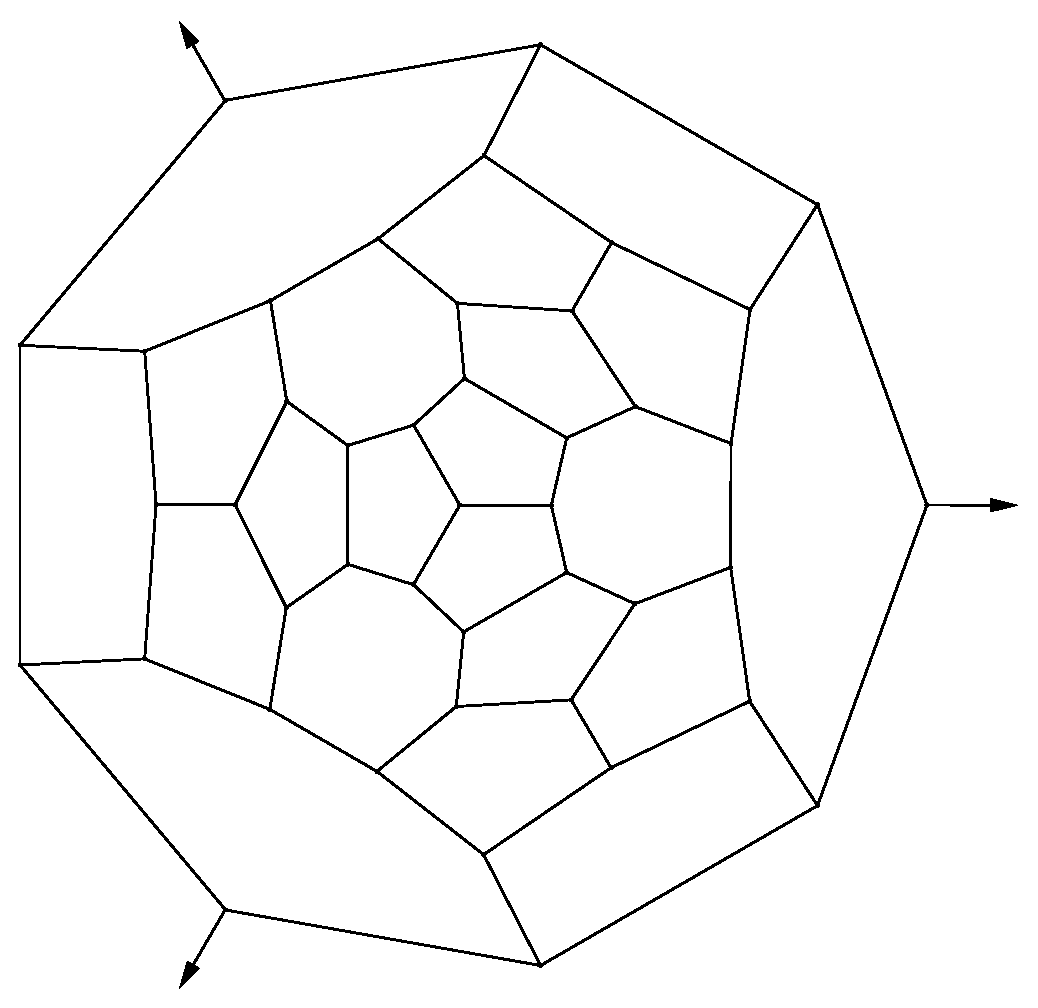
\includegraphics{5R3/Graph57_5R3_7R1sec.eps}}\par
$(5,7)$-sphere $5R_3$, $7R_1$
\end{minipage}
\begin{minipage}{4.7cm}
\centering
\resizebox{3.8cm}{!}{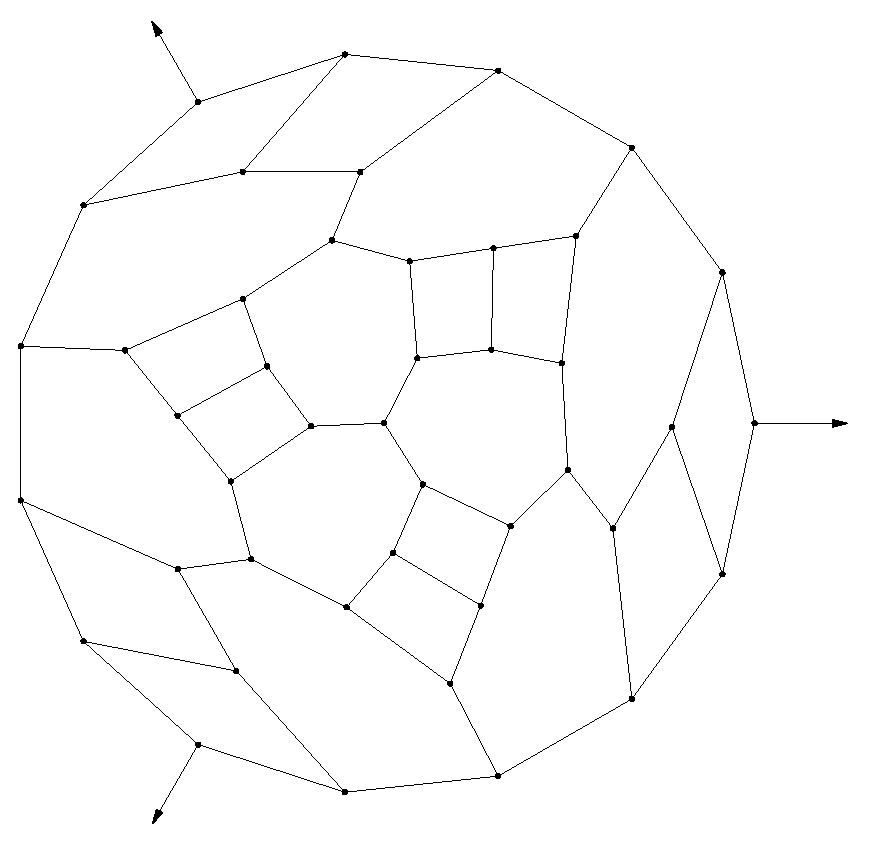
\includegraphics{FaceRegularPictures/FaceReg_4R1_7R4sec.eps}}\par
$(4,7)$-sphere $4R_1$, $7R_4$
\end{minipage}

\end{center}
\end{slide}







\begin{slide}{Euler formula}
\begin{itemize}
\item If $e_{p-q}$ denote the number of edges 
separating $p$- and $q$-gon, then one has:
\begin{equation*}
e_{p-q}=(p-i)f_p=(q-j)f_q
\end{equation*}
\item Euler formula $V-E+F=2-2g$ with $g$ being the genus,
can be rewritten as
\begin{equation*}
(6-p)f_p+(6-q)f_q=6(2-2g)
\end{equation*}
\item This implies
\begin{equation*}
e_{p-q}\textcolor{red}{\{\frac{6-p}{p-i}+\frac{6-q}{q-j}\} }=e_{p-q}\textcolor{red}{\alpha(p,q,i,j)}=12(1-g)
\end{equation*}
\end{itemize}


\end{slide}








\begin{slide}{A classification}
%Three cases are possible:
\vspace{-3mm}
\begin{itemize}
\item If \textcolor{red}{$\alpha(p,q,i,j)>0$}, then $g=0$, the map exists only on sphere and the number of vertices depends only on $\alpha(p,q,i,j)$.
\item If \textcolor{red}{$\alpha(p,q,i,j)=0$}, then $g=1$, the map exists only on torus.
\item If \textcolor{red}{$\alpha(p,q,i,j)<0$}, then $g>1$, the map exists only on surfaces of higher genus and the number of vertices is determined by the genus and $\alpha(p,q,i,j)$.
\end{itemize}
Detailed classification:
\begin{itemize}
\item \textcolor{red}{On sphere}: $55$ sporadic examples + two infinite series: $Prism_q$ and $Barrel_q$
\item \textcolor{red}{On torus}: $7$ sporadic examples + $16$ infinite cases.
\end{itemize}


\end{slide}



%\begin{slide}{List of tori}
%\begin{center}
%{\scriptsize
%\begin{tabular}{c|c|c|c|c|c|c}
%Nr.& str. Face Reg. &Nr of all & Tilings  \\
%\hline
%1&  $3R_0$, $7R_6$  &$\infty$ &$\frac{1}{6}$-truncated $(6^3)$   \\
%2&  $3R_0$, $8R_6$  &$\infty$ &$\frac{1}{3}$-truncated $(6^3)$  \\
%3&  $3R_0$, $9R_6$  &$\infty$ &$\frac{1}{2}$-truncated $(6^3)$  \\
%4&  $3R_0$, $10R_6$ &$\infty$ &$\frac{2}{3}$-truncated $(6^3)$  \\
%5&  $3R_0$, $11R_6$ &$\infty$ &$\frac{5}{6}$-truncated $(6^3)$   \\
%6&  $3R_0$, $12R_6$ &1        &trunc.$(6^3)=(3.12^2)$   \\ \hline
%7&  $4R_2$, $8R_6$  &$\infty$ &4-triakon of Nr.1   \\
%8&  $4R_2$, $10R_6$ &$\infty$ &4-triakon of Nr.2  \\
%9&  $4R_2$, $12R_6$ &$\infty$ &4-triakon of Nr.3   \\
%10& $4R_2$, $14R_6$ &$\infty$ &4-triakon of Nr.4   \\
%11& $4R_2$, $16R_6$ &$\infty$ &4-triakon of Nr.5   \\
%12& $4R_2$, $18R_6$ &1        &4-triakon of Nr.6  \\
%13& $4R_0$, $7R_5$  &$\infty$ &8-halved $(4.8^2)$    \\
%14& $4R_0$, $8R_4$  &1        &trunc.$(4^4)=(4.8^2)$   \\
%15& $4R_1$, $8R_5$  &$\infty$ &4-halved Nr.13   \\
%16& $4R_1$, $10R_4$ &$\infty$ &4-halved $(4.8^2)$   \\ \hline
%17& $5R_1$, $7R_3$  &$\infty$ &a 6-halved $(6^3)$   \\
%18& $5R_2$, $7R_4$  &$1+\infty$ &decorated $(6^3)$  \\
%19& $5R_2$, $8R_2$  &$\infty$ &a 6-halved $(6^3)$  \\
%20& $5R_3$, $8R_4$  &1        &decorated $(6^3)$  \\
%21& $5R_3$, $10R_2$ &1        &decorated $(6^3)$  \\
%22& $5R_3$, $11R_1$ &1        &decorated $(6^3)$  \\
%23& $5R_3$, $12R_0$ &1        &a 5-triakon $(6^3)$  \\ \hline
%\end{tabular}
%}
%\end{center}
%
%\end{slide}














\begin{slide}{Some sporadic spheres}
\vspace{-3mm}
\begin{center}
\begin{minipage}{5.1cm}
\centering
\resizebox{3.3cm}{!}{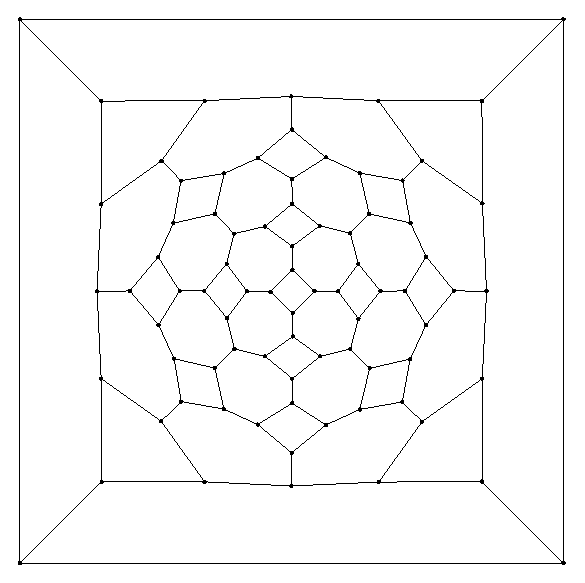
\includegraphics{FaceRegularPictures/FaceReg_4R0_7R4_2.eps}}\par
$(4,7)$-sphere $4R_0$, $7R_4$
\end{minipage}
\begin{minipage}{5.1cm}
\centering
\resizebox{3.3cm}{!}{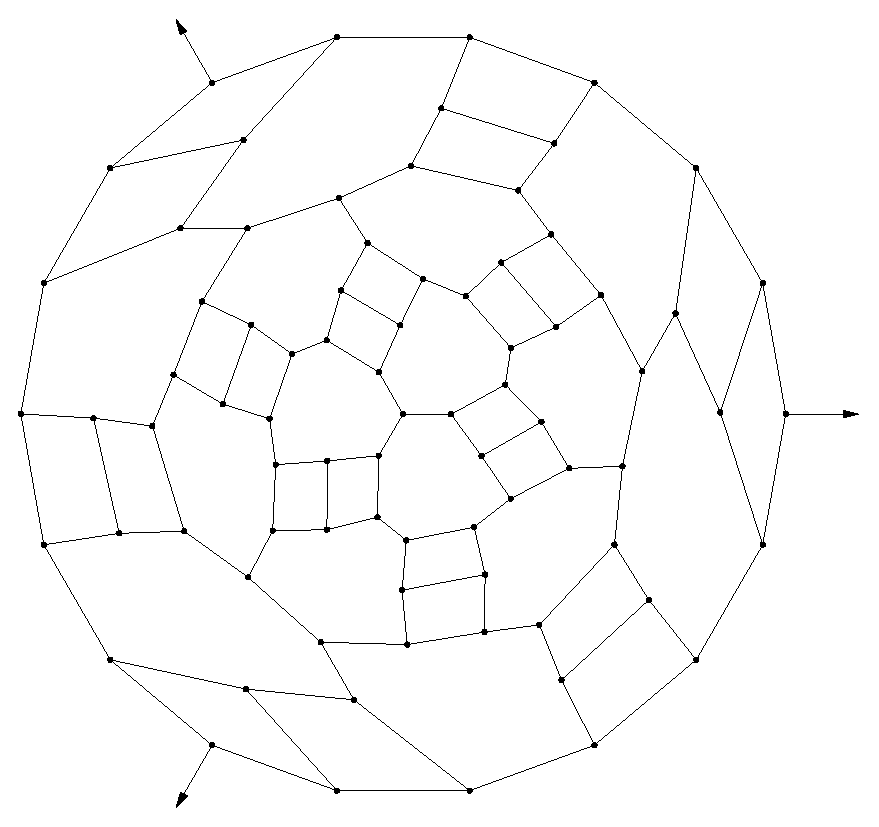
\includegraphics{Picture48_8R4/WP2_1thi.eps}}\par
$(4,8)$-sphere $4R_1$, $8R_4$
\end{minipage}
\begin{minipage}{5.1cm}
\centering
\resizebox{3.3cm}{!}{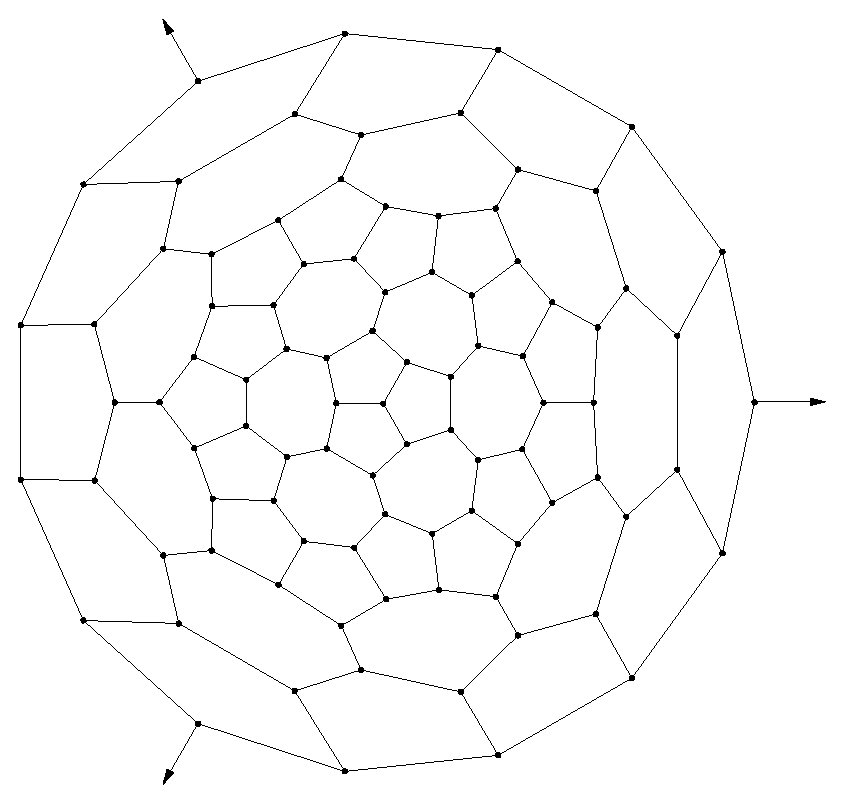
\includegraphics{FaceRegularPictures/FaceReg_5R2_7R2sec.eps}}\par
$(5,7)$-sphere $5R_2$, $7R_2$
\end{minipage}
\begin{minipage}{5.1cm}
\centering
\resizebox{3.3cm}{!}{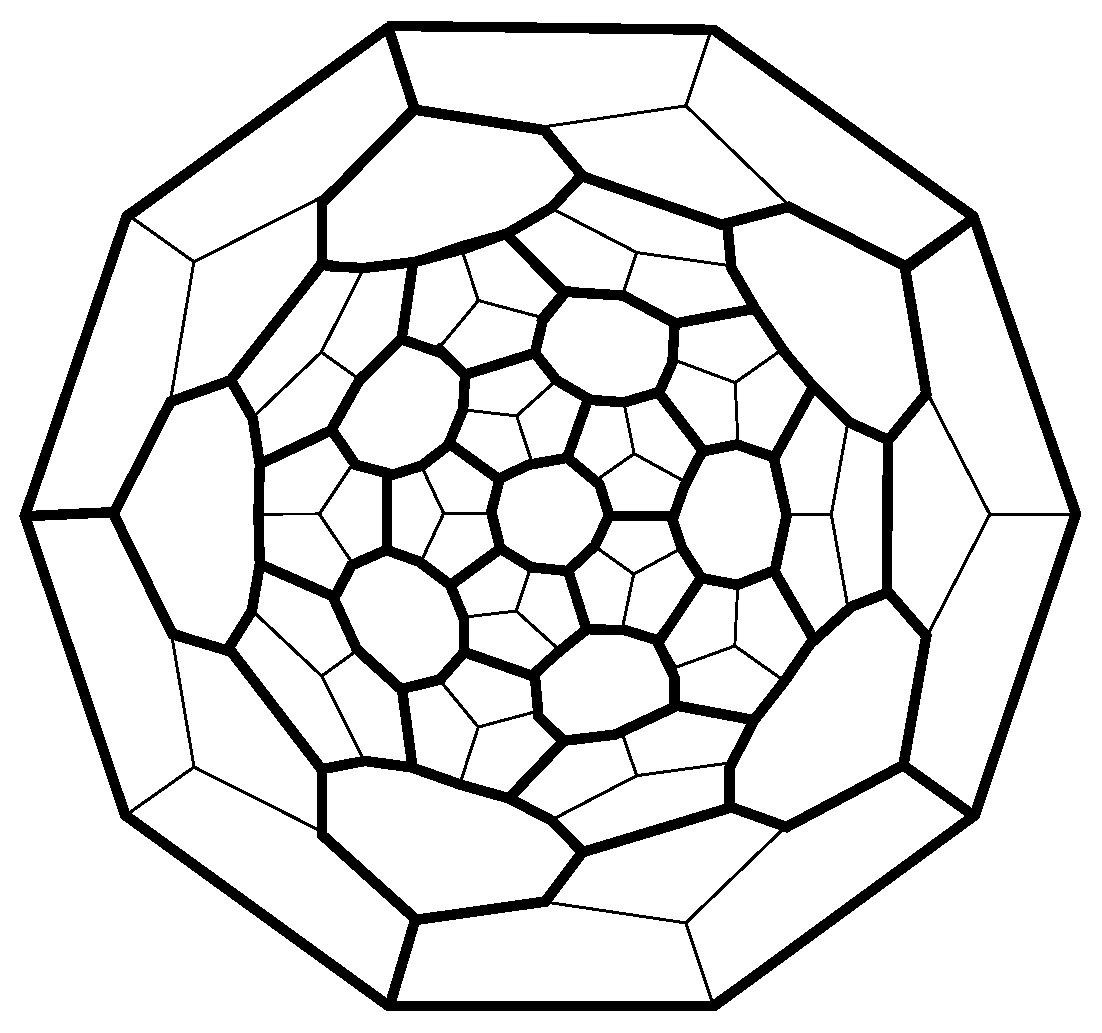
\includegraphics{FaceRegularPictures/60sec.eps}}\par
$(5,10)$-sphere $5R_3$, $10R_0$
\end{minipage}
\end{center}

\end{slide}








\overlays{2}{
\begin{slide}{Sporadic tori}
\onlySlide*{1}{
\vspace{-6mm}
\begin{center}
\begin{minipage}{5.1cm}
\centering
\resizebox{4.3cm}{!}{\includegraphics[bb=150 286 476 540, clip]{FaceRegularPictures/UniqueTorus312_12R6.eps}}\par
$(3,12)$-torus $3R_0$, $12R_6$
\end{minipage}
\begin{minipage}{5.1cm}
\centering
\resizebox{4.3cm}{!}{\includegraphics[bb=150 286 476 540, clip]{FaceRegularPictures/UniqueTorus48_8R4.eps}}\par
$(4,8)$-torus $4R_0$, $8R_4$
\end{minipage}
\begin{minipage}{5.1cm}
\centering
\resizebox{4.3cm}{!}{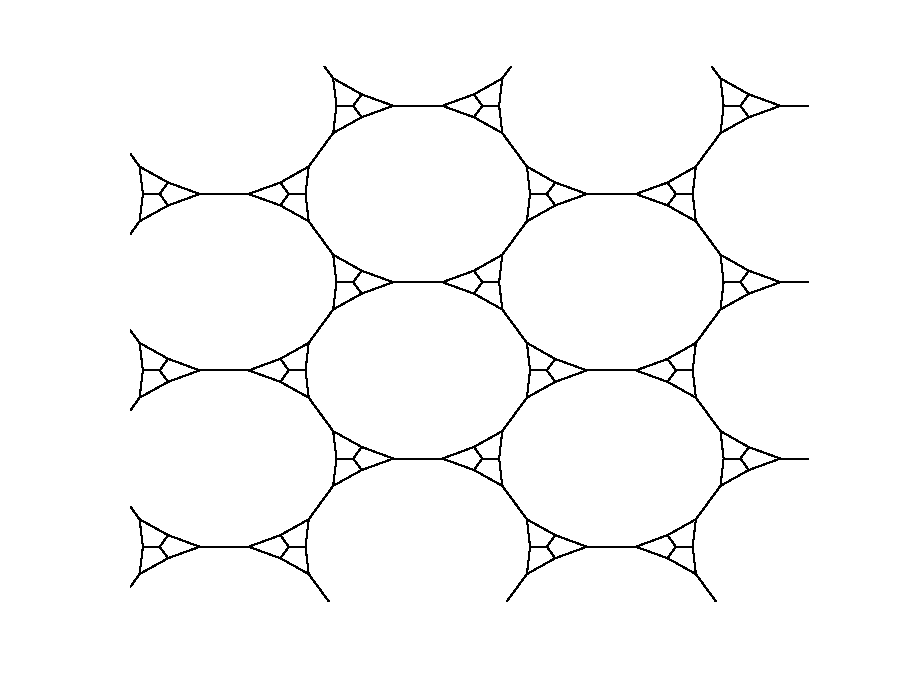
\includegraphics[bb=150 286 476 540, clip]{FaceRegularPictures/Torus418_4R2_18R6.eps}}\par
$(4,18)$-torus $4R_2$, $18R_6$
\end{minipage}
\end{center}
}
\onlySlide*{2}{
\vspace{-6mm}
\begin{center}
\begin{minipage}{5.1cm}
\centering
\resizebox{4.3cm}{!}{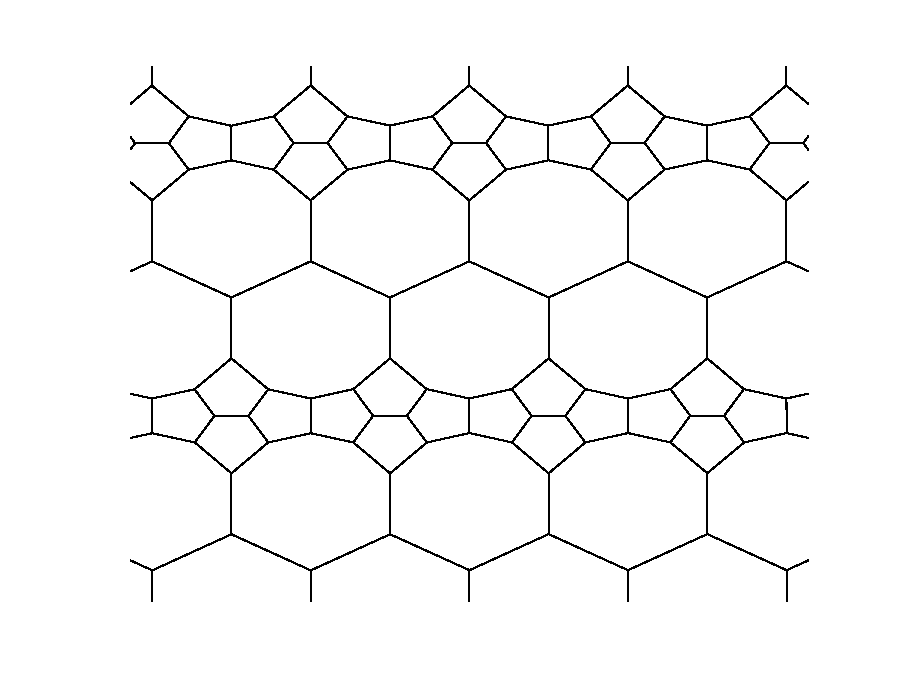
\includegraphics[bb=150 286 476 540, clip]{FaceRegularPictures/UniqueStrictly8R4_5R3.eps}}\par
$(5,8)$-torus $5R_3$, $8R_4$
\end{minipage}
\begin{minipage}{5.1cm}
\centering
\resizebox{4.3cm}{!}{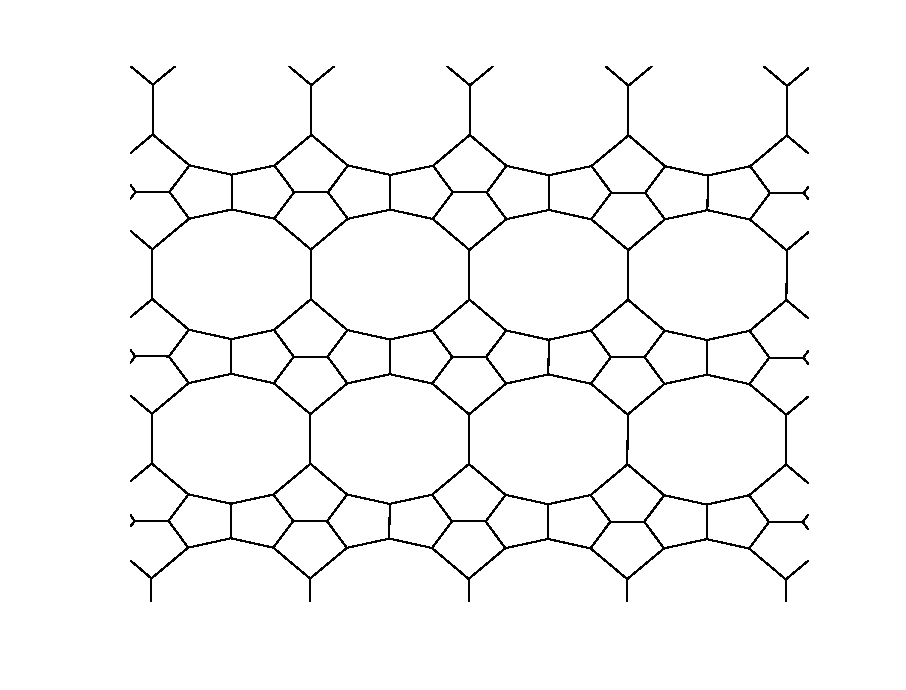
\includegraphics[bb=150 286 476 540, clip]{FaceRegularPictures/UniqueStrictly10R2_5R3.eps}}\par
$(5,10)$-torus $5R_3$, $10R_2$
\end{minipage}
\begin{minipage}{5.1cm}
\centering
\resizebox{4.3cm}{!}{\includegraphics[bb=150 286 476 540, clip]{FaceRegularPictures/UniqueStrictly11R1_5R3.eps}}\par
$(5,11)$-torus $5R_3$, $11R_1$
\end{minipage}
\begin{minipage}{5.1cm}
\centering
\resizebox{4.3cm}{!}{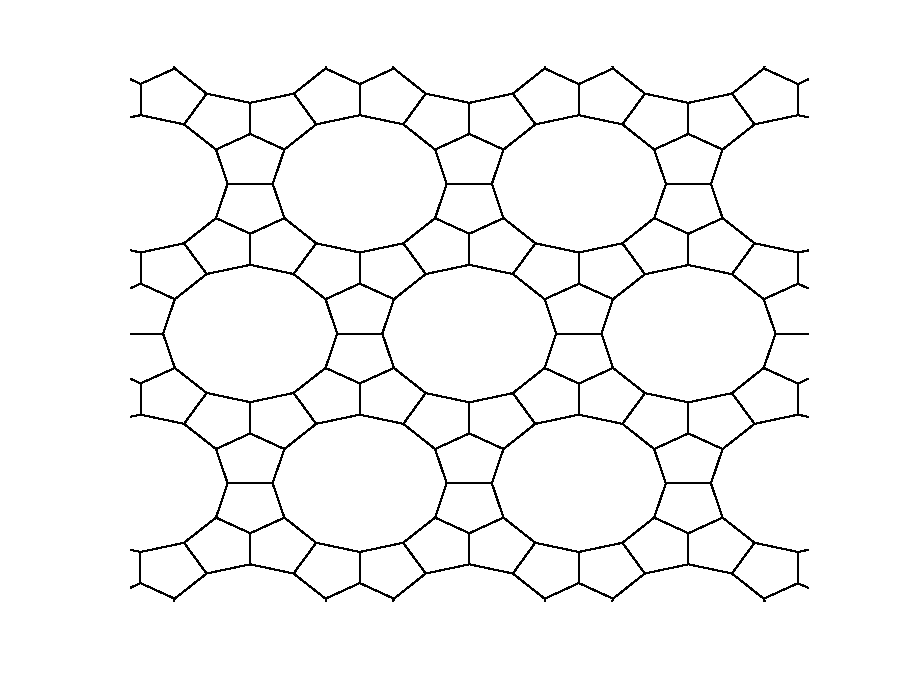
\includegraphics[bb=150 286 476 540, clip]{FaceRegularPictures/UniqueStrictly12R0_5R3.eps}}\par
$(5,12)$-torus $5R_3$, $12R_0$
\end{minipage}
\end{center}
}
\end{slide}
}










\begin{slide}{$(3,q)$-tori $3R_0$, $qR_6$ {\small $(7 \le q \le 12)$}}
\begin{itemize}
\item They are obtained by truncating 
a $3$-valent tesselation of the torus by $6$-gons on the vertices
from a set $S_q$,
such that every face is incident to exactly $q-6$ vertices in $S_q$.
\item There is an infinity of possibilities, except for $q=12$.
\begin{center}
\begin{minipage}{3.5cm}
\centering
\resizebox{3.3cm}{!}{\includegraphics[bb=150 266 476 540, clip]{StrictTorus3R0/Torus37_3R0_7R6_1.eps}}\par
$(3,7)$-torus $3R_0$, $7R_6$
\end{minipage}
\begin{minipage}{3.5cm}
\centering
\resizebox{3.3cm}{!}{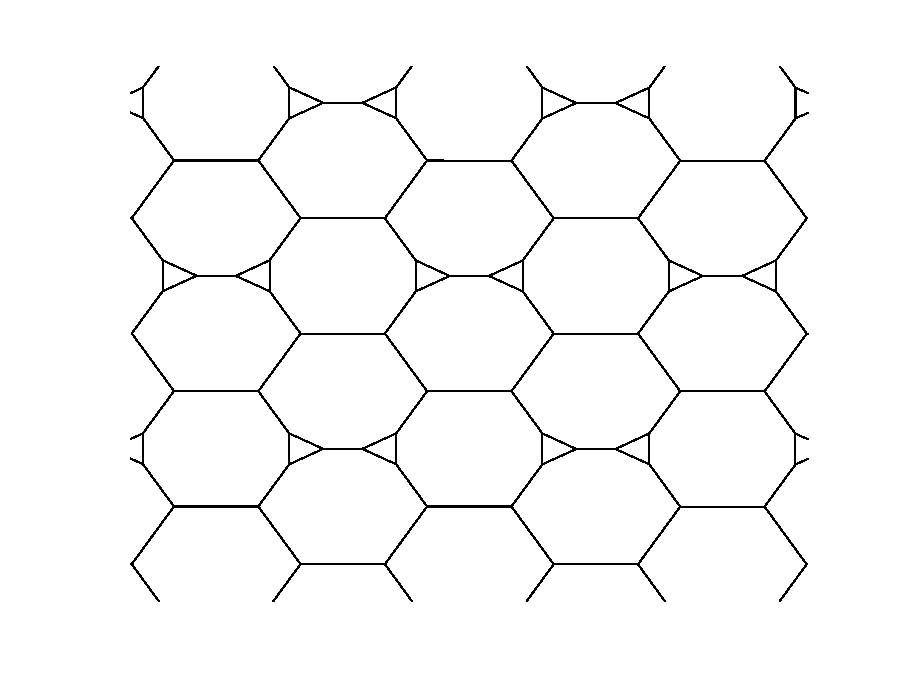
\includegraphics[bb=150 266 476 540, clip]{StrictTorus3R0/Torus38_3R0_8R6_1.eps}}\par
$(3,8)$-torus $3R_0$, $8R_6$
\end{minipage}
\begin{minipage}{3.5cm}
\centering
\resizebox{3.3cm}{!}{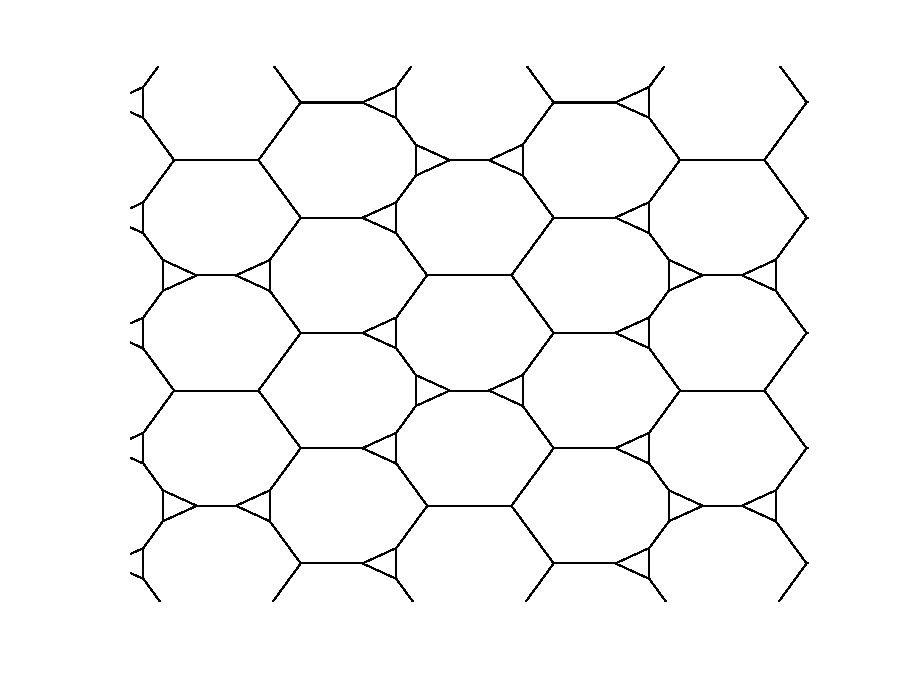
\includegraphics[bb=150 266 476 540, clip]{StrictTorus3R0/Torus39_3R0_9R6_10.eps}}\par
$(3,9)$-torus $3R_0$, $9R_6$
\end{minipage}
\end{center}
\item $(4,q)$-tori $4R_2$, $qR_6$ ($4 \le \frac{q}{2} \le 9$)
are obtained (from 6 above) by $4$-triakon (dividing $3$-gon into triple of $4$-gons)

\end{itemize}
\end{slide}







\begin{slide}{$(4,10)$-tori $4R_1$, $10R_4$}
\begin{itemize}
\item Take the symbols
\begin{center}
\begin{minipage}{5.3cm}
\centering
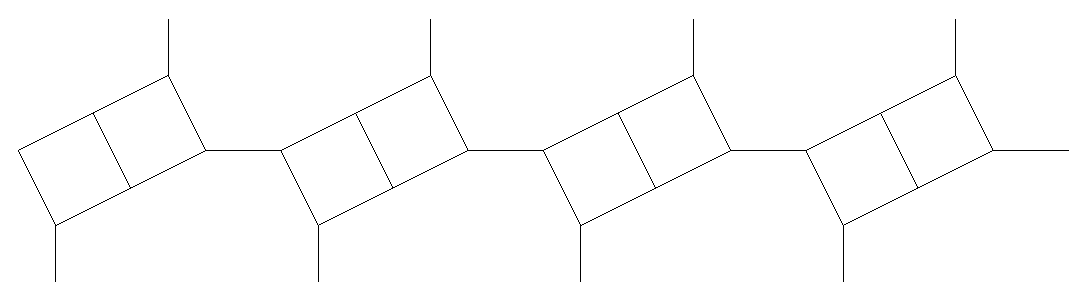
\epsfig{height=12mm, file=FaceRegularPresPic/RedCont16_1.eps}\par
$u$
\end{minipage}
\begin{minipage}{5.3cm}
\centering
\epsfig{height=12mm, file=FaceRegularPresPic/RedCont16_2.eps}\par
$v$
\end{minipage}
\end{center}
\item The torus correspond to words of the form $(\alpha_0\dots\alpha_n)^{\infty}$ with $\alpha_i$ being equal to $u$ or $v$.
\begin{center}
\begin{minipage}{5.2cm}
\centering
\resizebox{4.5cm}{!}{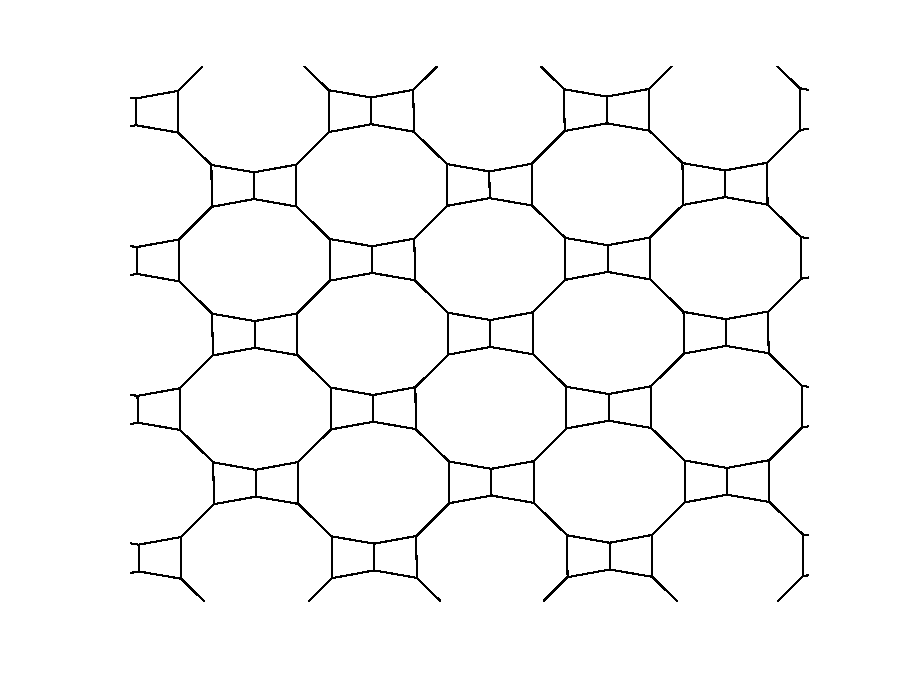
\includegraphics[bb=150 330 476 540, clip]{FaceRegularPictures/Torus410_4R1_10R4_14.eps}}\par
$(u)^{\infty}$
\end{minipage}
\begin{minipage}{5.2cm}
\centering
\resizebox{4.5cm}{!}{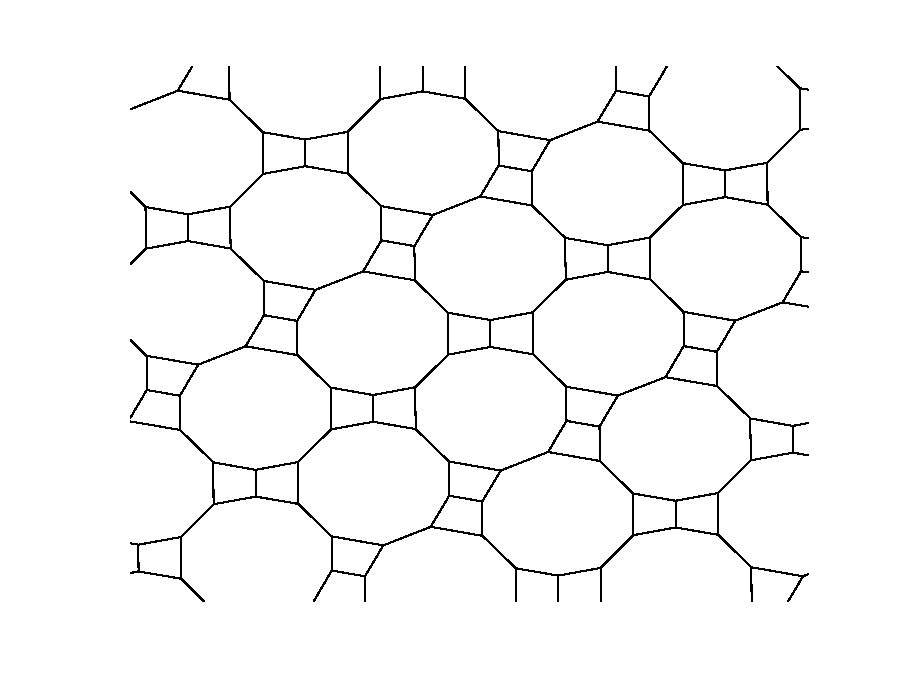
\includegraphics[bb=150 330 476 540, clip]{FaceRegularPictures/Torus410_4R1_10R4_16.eps}}\par
$(uv)^{\infty}$
\end{minipage}
\end{center}

\end{itemize}
\end{slide}


\begin{slide}{$(5,7)$-tori $5R_1$, $7R_3$}
\begin{itemize}
\item Take the symbols
\begin{center}
\begin{minipage}{5.3cm}
\centering

\epsfig{height=13mm, file=FaceRegularPresPic/RedCont17_1.eps}\par
$u$
\end{minipage}
\begin{minipage}{5.3cm}
\centering
\epsfig{height=13mm, file=FaceRegularPresPic/RedCont17_2.eps}\par
$v$
\end{minipage}
\end{center}
\item The torus correspond to words of the form $(\alpha_0\dots\alpha_n)^{\infty}$ with $\alpha_i$ being equal to $u$ or $v$.
\begin{center}
\begin{minipage}{5.2cm}
\centering
\resizebox{4.0cm}{!}{\includegraphics[bb=150 310 476 540, clip]{FaceRegularPictures/Torus57_5R1_1.eps}}\par
$(u)^{\infty}$
\end{minipage}
\begin{minipage}{5.2cm}
\centering
\resizebox{4.0cm}{!}{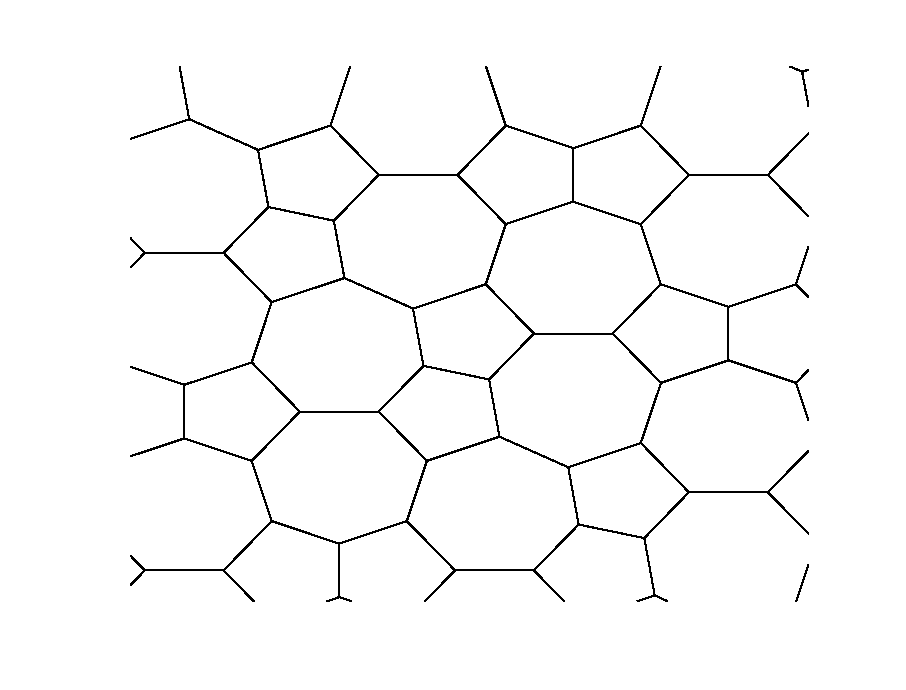
\includegraphics[bb=150 310 476 540, clip]{FaceRegularPictures/Torus57_5R1_2.eps}}\par
$(uv)^{\infty}$
\end{minipage}
\end{center}

\end{itemize}
\end{slide}









\overlays{2}{
\begin{slide}{$(5,7)$-tori $5R_2$, $7R_4$}
\onlySlide*{1}{
\begin{itemize}
\item If $5$-gons form infinite lines, then \textcolor{red}{one possibility}:
\begin{center}
\begin{minipage}{5.2cm}
\centering
\resizebox{4.0cm}{!}{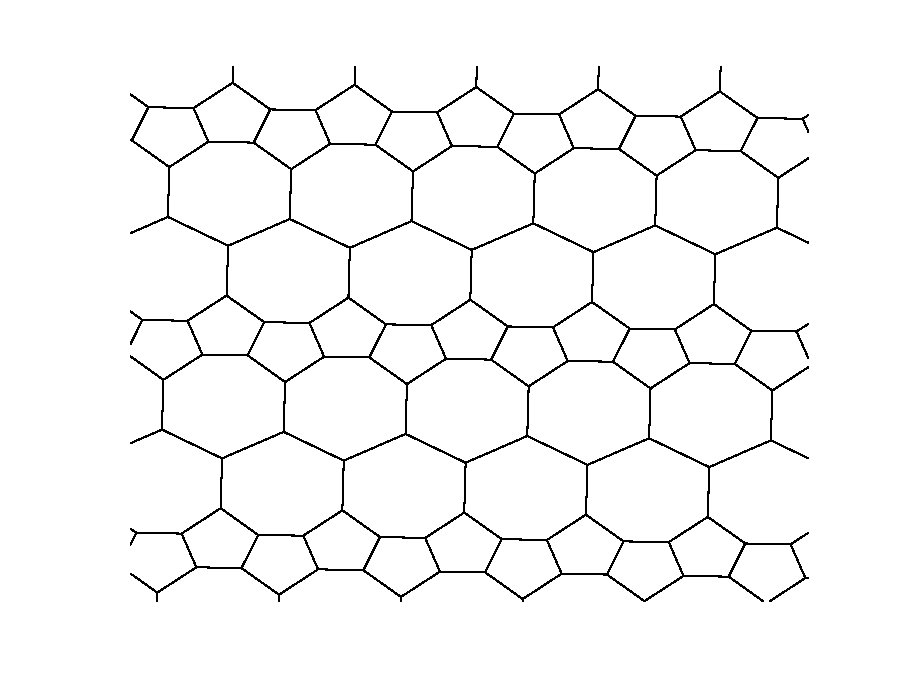
\includegraphics[bb=150 350 476 540, clip]{FaceRegularPictures/Unique57_LinesOf2.eps}}\par
\end{minipage}
\end{center}
\item Take the symbols
\begin{center}
\begin{minipage}{5.2cm}
\centering

\epsfig{height=13mm, file=FaceRegularPresPic/RedCont18_1.eps}\par
$u$
\end{minipage}
\begin{minipage}{5.2cm}
\centering

\epsfig{height=13mm, file=FaceRegularPresPic/RedCont18_2.eps}\par
$v$
\end{minipage}
\end{center}
\end{itemize}
}
\onlySlide*{2}{
\begin{itemize}
\item Other tori correspond to words of the form $(\alpha_0\dots\alpha_n)^{\infty}$ with $\alpha_i$ being equal to $u$ or $v$.
\begin{center}
\begin{minipage}{5.2cm}
\centering
\resizebox{5.0cm}{!}{\includegraphics[bb=150 266 476 540, clip]{FaceRegularPictures/Torus57_5R2_7R4_u.eps}}\par
$(u)^{\infty}$
\end{minipage}
\begin{minipage}{5.2cm}
\centering
\resizebox{5.0cm}{!}{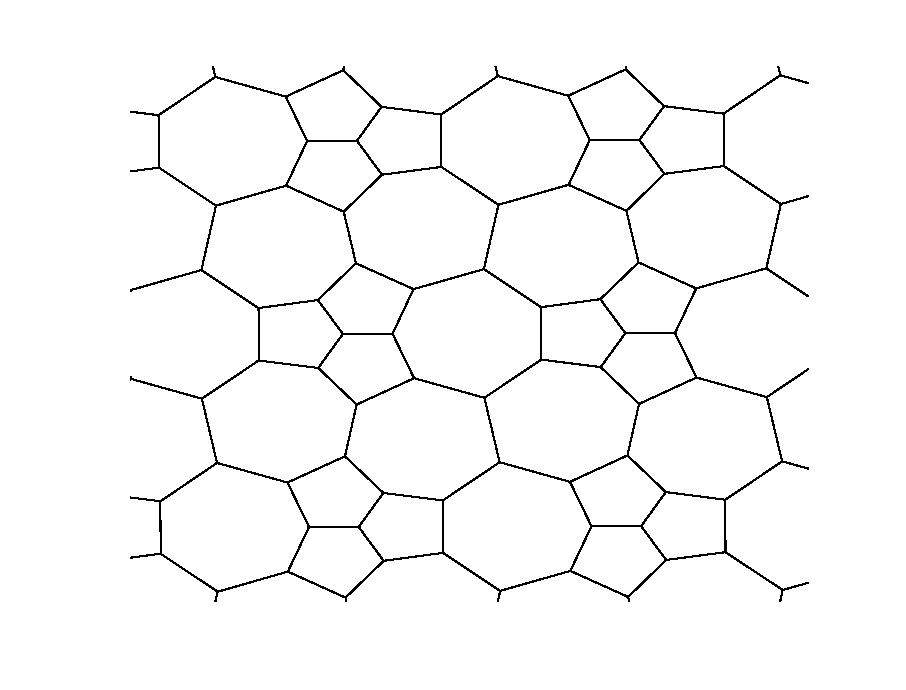
\includegraphics[bb=150 266 476 540, clip]{FaceRegularPictures/Torus57_5R2_7R4_uv.eps}}\par
$(uv)^{\infty}$
\end{minipage}
\end{center}
\end{itemize}
}
\end{slide}
}



\begin{slide}{$(5,8)$-tori $5R_2$, $8R_2$}
\begin{itemize}
\item $5$-gons and $8$-gons are organized in infinite lines.
\item Only two configurations for $5$-gons locally:
\begin{center}
\begin{minipage}{5.2cm}
\centering
\epsfig{height=13mm, file=FaceRegularPresPic/3_5_polycycle_1.eps}\par
$u$
\end{minipage}
\begin{minipage}{5.2cm}
\centering
\epsfig{height=13mm, file=FaceRegularPresPic/3_5_polycycle_2.eps}\par
$v$
\end{minipage}
\end{center}
\item Words of the form $(\alpha_0\dots\alpha_n)^{\infty}$ with $\alpha_i$ being equal to $uv$ or $vu$.
\begin{center}
\begin{minipage}{5.2cm}
\centering
\resizebox{4.0cm}{!}{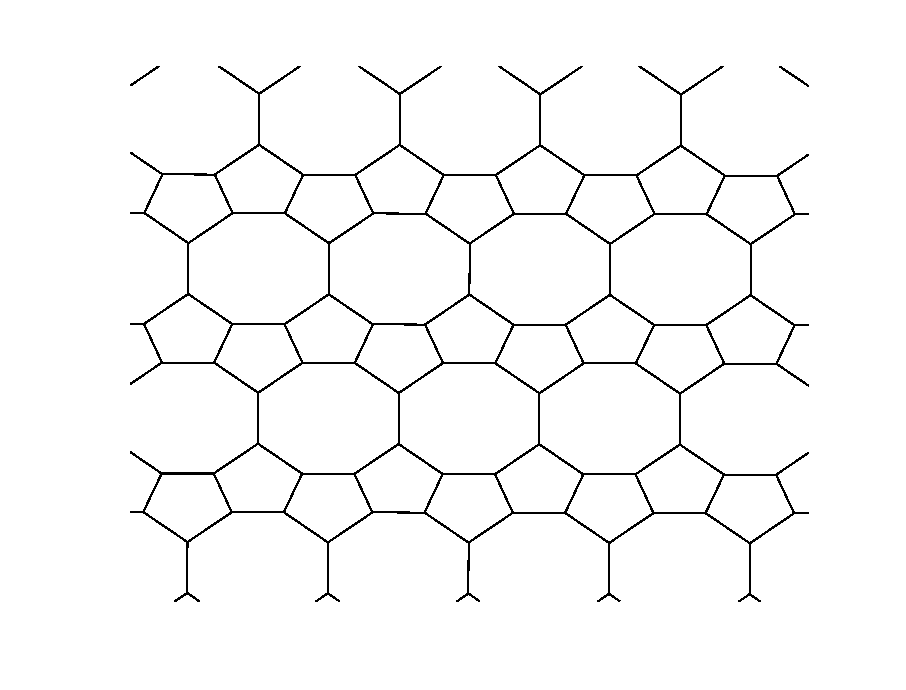
\includegraphics[bb=150 370 476 540, clip]{FaceRegularPictures/Torus58_5R2_3.eps}}\par
$(uv)^{\infty}$
\end{minipage}
\begin{minipage}{5.2cm}
\centering
\resizebox{4.0cm}{!}{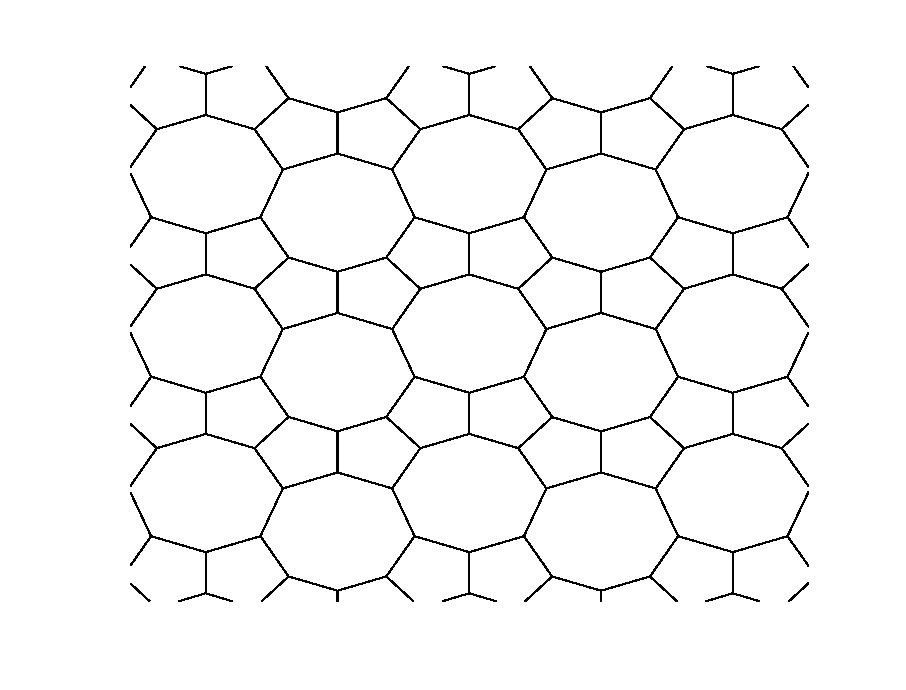
\includegraphics[bb=150 370 476 540, clip]{FaceRegularPictures/Torus58_5R2_2.eps}}\par
$(uvvu)^{\infty}$
\end{minipage}
\end{center}


\end{itemize}
\end{slide}



\overlays{2}{
\begin{slide}{$(4,8)$-tori $4R_1$, $8R_5$}
\fromSlide{1}{
\begin{itemize}
\item They are in one-to-one correspondence with \textcolor{red}{perfect matchings} \textcolor{red}{$PM$} of a $6$-regular triangulation of the torus, such that every vertex is contained in a triangle, whose edge, opposite to this vertex, belongs to \textcolor{red}{$PM$}.

\end{itemize}
}%
\onlySlide*{1}{
\begin{center}
\begin{minipage}{9.2cm}
\centering
\resizebox{9.0cm}{!}{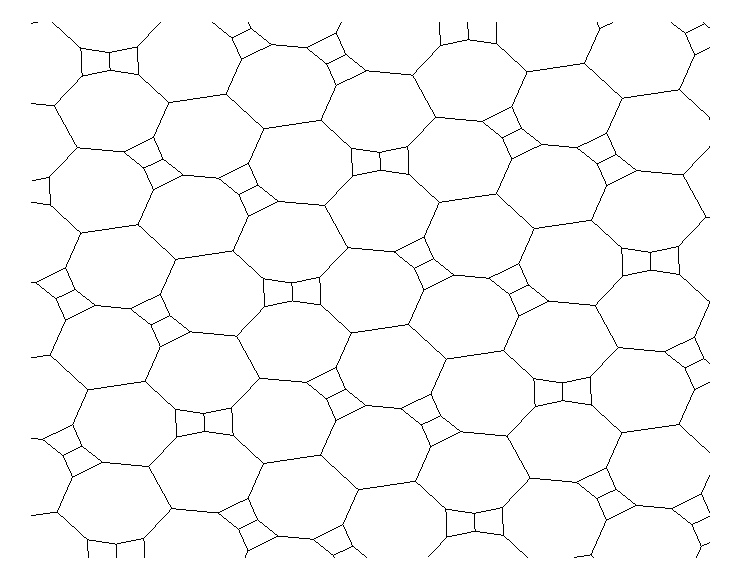
\includegraphics[bb=0 80 336 261, clip]{FaceRegularPresPic/Torus48_4R1_8R5_5_BS.eps}}\par
\end{minipage}
\end{center}
}%
\onlySlide*{2}{
\begin{center}
\begin{minipage}{9.2cm}
\centering
\resizebox{9.0cm}{!}{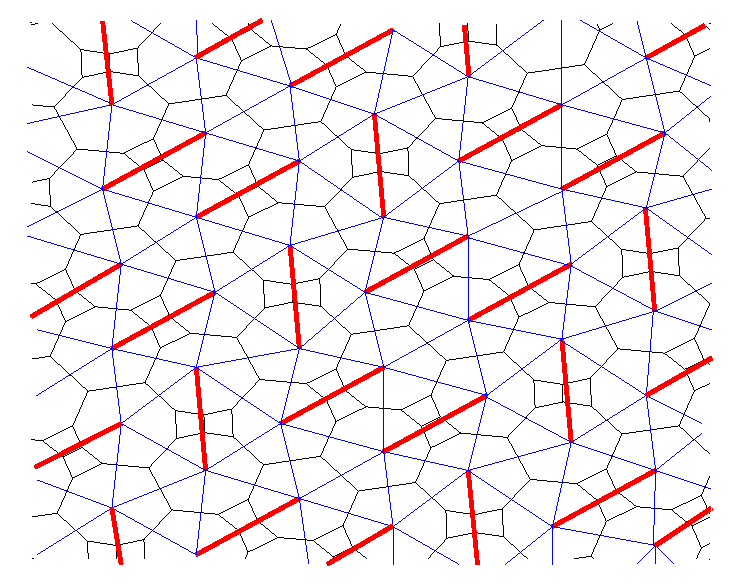
\includegraphics[bb=0 80 336 261, clip]{FaceRegularPresPic/Torus48_4R1_8R5_5_PM.eps}}\par
\end{minipage}
\end{center}
}%

\end{slide}
}





\begin{slide}{$(4,7)$-tori $4R_0$, $7R_5$}
\begin{itemize}
\item Given a $(4,8)$-torus, which is $4R_1$ and $8R_5$, the removal of edges between two $4$-gons produces a $(4,7)$-torus, which is $4R_0$ and $7R_5$.
\item Any such $(4,7)$-torus can be obtained in this way from two $(4,8)$-tori $T_1$ and $T_2$, which are $4R_1$ and $8R_5$.
\item $T_1$ and $T_2$ are obtained from each other by the transformation
\begin{center}
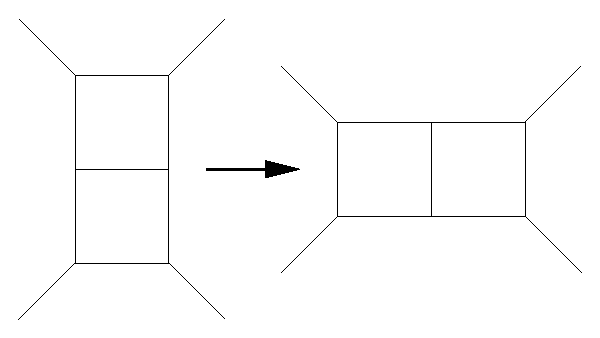
\epsfig{file=FaceRegularPictures/FlippingPairSquare.eps, height=4cm}
\end{center}



%Infinity but this case is not classified.
%\item The following example shows the difficulty of a classification.
%\begin{center}
%\begin{minipage}{8.2cm}
%\centering
%\resizebox{8.0cm}{!}{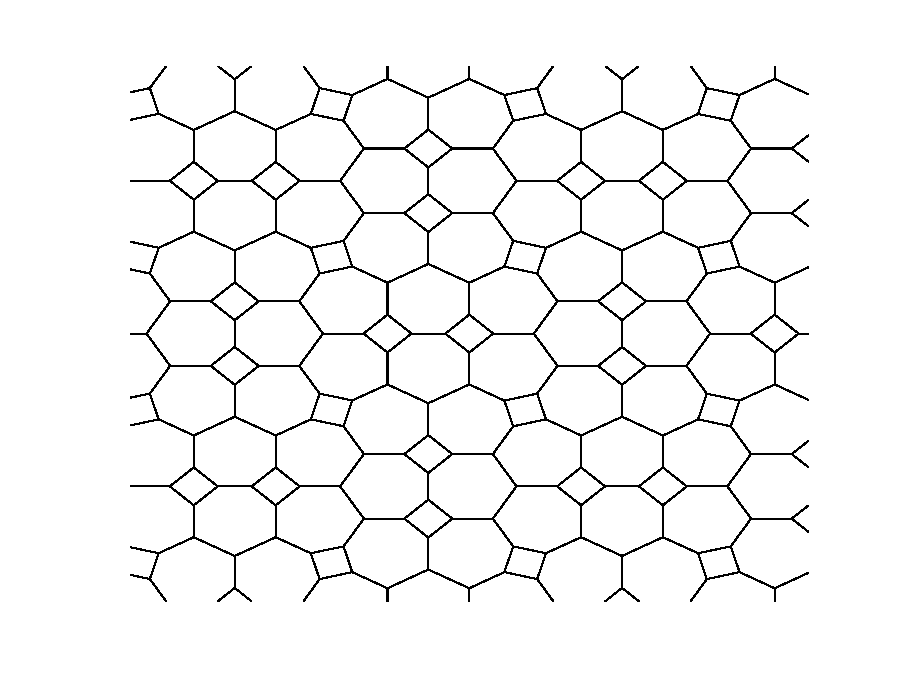
\includegraphics[bb=150 320 476 540, clip]{Torus47_4R0_7R5_22.eps}}\par
%\end{minipage}
%\end{center}

\end{itemize}
\end{slide}



\begin{slide}{Our research program}
\begin{itemize}
\item We investigated the cases of $3$-regular spheres and tori being
$pR_i$ or $qR_j$.
\item Such maps with $q=6$ should be on sphere only.
\begin{itemize}
\item All $(3,6)$-spheres are $3R_0$.
\item There are infinities of $(4,6)$-spheres $4R_i$ for $i=0$, $1$, $2$; there are $9$ $(4,6)$-spheres $6R_j$.
\item There are infinities of $(5,6)$-spheres $5R_i$ for $i=0$, $1$, $2$; there are two spheres $5R_3$ and $26$ spheres $6R_j$.
\end{itemize}
So, we will assume $q\geq 7$.
%All such maps with $q=6$ are given by Deza \& Grishukhin:
%\item We do not considered the cases of $q=6$, since in that case the
%number of $p$-gonal faces is fixed and this has already been considered.
%\item We do not consider the case of $(3,q)$-map for lack of time.
\item For a $(p,q)$-polyhedron, which is $qR_j$, one has $j\leq 5$.
\item For a $3$-connected $(p,q)$-torus, which is $qR_j$,
one has $j\leq 6$.

\end{itemize}
\end{slide}

\begin{slide}{Representations of $(p,q)$-maps}
\begin{itemize}
\item \textcolor{red}{Steinitz theorem}: Any $3$-connected planar graph is the skeleton of a polyhedron.
\item \textcolor{red}{Torus case}:
\begin{itemize}
\item A $(p,q)$-torus has a fundamental group isomorphic to $\ZZ^2$, its universal cover is a periodic $(p,q)$-plane.
\item A periodic $(p,q)$-plane is the universal cover of an infinity of $(p,q)$-tori.
\item Take a $(p,q)$-torus $T$ and its corresponding $(p,q)$-plane $P$.
If all translation preserving $P$ arise from the fundamental group of $T$,
then $T$ is called \textcolor{red}{minimal}.
\item Any $(p,q)$-plane is the universal cover of a \textcolor{red}{unique} minimal torus.
\end{itemize}



\end{itemize}
\end{slide}



\begin{slide}{}
\begin{center}
{\Huge 
\begin{tabular*}{7cm}{c}
\\[-0.5cm]
\textcolor{blue}{II. }\textcolor{red}{$(p,3)$-polycycles}
\end{tabular*}
}
\end{center}
\end{slide}



%$G$ of girth $p$ and maximal vertex-degree $s$, which admits
%a realization on the plane, such that:

\begin{slide}{$(p,3)$-polycycles}
A \textcolor{red}{generalized $(p,3)$-polycycle} is a 
$2$-connected plane graph with faces partitioned
in two families $F_1$ and $F_2$, so that:
\begin{itemize}
\item all elements of $F_1$ (\textcolor{red}{proper faces}) are
(combinatorial) $p$-gons;
\item all elements of $F_2$ (\textcolor{red}{holes}, the exterior face
is amongst them) are pairwisely disjoint;
\item all vertices have valency $3$ or $2$ and any $2$-valent vertex lies on a 
boundary of a hole.
%\item A $(5,3)$-polycycle: if the exterior face is the unique hole.
\end{itemize}

\begin{center}
\epsfig{file=FaceRegularPresPic/PolycycleFig2.eps, height=2cm}
\end{center}

\end{slide}





\begin{slide}{$(3,3)$ and $(4,3)$-polycycles}
{\it\scriptsize

%{\bf Theorem}

(i) \textcolor{red}{Any $(3,3)$-polycycle} is one of the following $3$ cases:
\begin{center}
\epsfig{figure=Boundary/Possible3gonalPatchNOB.eps,width=6cm}
\end{center}

(ii) \textcolor{red}{Any $(4,3)$-polycycle} belongs to the following $3$ cases:
\begin{center}
\epsfig{figure=FaceRegularPresPic/Discrete4gonal_SEC.eps,width=6cm}
\end{center}
\hspace{1cm}or belong to the following infinite family of $(4,3)$-polycycles:
\begin{center}
\epsfig{figure=Boundary/InfiniteSequenceNOB.eps,width=8cm}
\end{center}

}
This classification is very useful for classifying $(4,q)$-maps.

\end{slide}





\overlays{6}{
\begin{slide}{$(5,3)$-polycycle decomposition}
\onlySlide*{1}{
A \textcolor{red}{bridge} is an edge going from a hole to a hole (possibly, the same).\\[1.3cm]
\begin{center}
\resizebox{6cm}{!}{\includegraphics{FaceRegularPresPic/PolycycleFig3.eps}}
\end{center}
}
\onlySlide*{2}{
Any generalized $(p,3)$-polycycle is \textcolor{red}{uniquely decomposable} along its bridges.
\begin{center}
\resizebox{9cm}{!}{\includegraphics{FaceRegularPresPic/PolycycleFig4.eps}}
\end{center}
}
\onlySlide*{3}{
%\textcolor{red}{Thm.}
The set of \textcolor{red}{non-decomposable} $(5,3)$-polycycles has been classified:
\begin{center}
\begin{minipage}{3.7cm}
\centering
\resizebox{3.0cm}{!}{\includegraphics{PictureAppli/Dodecahedron.eps}}\par
\end{minipage}
\begin{minipage}{3.7cm}
\centering
\resizebox{3.0cm}{!}{\rotatebox{90}{\includegraphics{Polycycle/PolycycleA2.eps}}}\par
\end{minipage}
\begin{minipage}{3.7cm}
\centering
\resizebox{3.0cm}{!}{\includegraphics{Polycycle/Dodecahedron3vertDegTwo.ps}}\par
\end{minipage}
\begin{minipage}{3.7cm}
\centering
\resizebox{3.0cm}{!}{\includegraphics{Polycycle/PolycycleA4.eps}}\par
\end{minipage}
\begin{minipage}{3.7cm}
\centering
\resizebox{3.0cm}{!}{\rotatebox{90}{\includegraphics{Polycycle/PolycycleB3sec.eps}}}\par
\end{minipage}
\begin{minipage}{3.7cm}
\centering
\resizebox{3.0cm}{!}{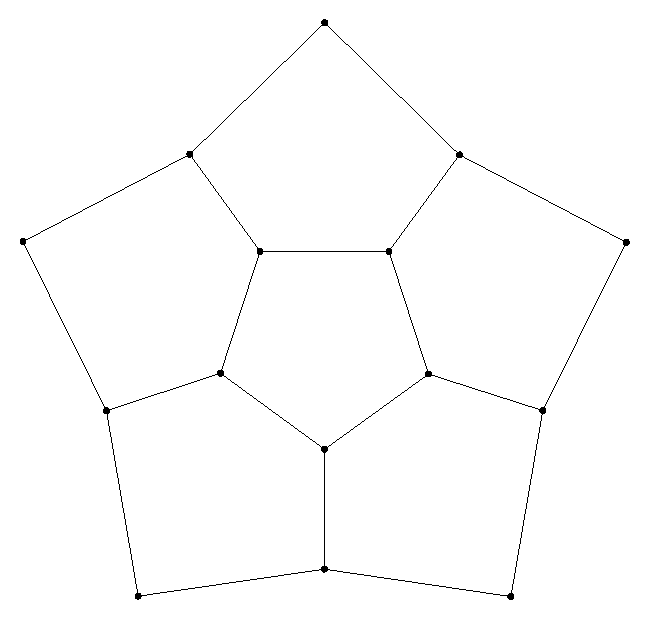
\includegraphics{Polycycle/PolycycleA5.eps}}\par
\end{minipage}
\end{center}
}
\onlySlide*{4}{
\begin{center}
\begin{minipage}{3.7cm}
\centering
\resizebox{3.0cm}{!}{\includegraphics{Polycycle/Fundamental22polycycle3.eps}}\par
\end{minipage}
\begin{minipage}{3.7cm}
\centering
\resizebox{3.0cm}{!}{\includegraphics{Polycycle/PolycycleB2.eps}}\par
\end{minipage}
\begin{minipage}{3.7cm}
\centering
\resizebox{2.5cm}{!}{\includegraphics{Polycycle/Elementary53_C2.eps}}\par
\end{minipage}
\begin{minipage}{3.7cm}
\centering
\resizebox{3.0cm}{!}{\includegraphics{Polycycle/Fundamental22polycycle2.eps}}\par
\end{minipage}
\begin{minipage}{3.7cm}
\centering
\resizebox{2.0cm}{!}{\rotatebox{180}{\includegraphics{Polycycle/PolycycleD.eps}}}\par
\end{minipage}

\end{center}
}
\onlySlide*{5}{
The \textcolor{red}{infinite series} of non-decomposable 
$(5,3)$-polycycles $E_n, n \ge 1$:\\[1cm]
\begin{center}
\begin{minipage}{3.7cm}
\centering
\epsfig{height=14mm, file=Polycycle/Elementary53_E1.eps}\par
\end{minipage}
\begin{minipage}{4.7cm}
\centering
\epsfig{height=14mm, file=Polycycle/Elementary53_E2.eps}\par
\end{minipage}
\end{center}
\vspace{1cm}
\begin{center}
\begin{minipage}{4.7cm}
\centering
\epsfig{height=14mm, file=Polycycle/Elementary53_E3.eps}\par
\end{minipage}
\begin{minipage}{4.7cm}
\centering
\epsfig{height=14mm, file=Polycycle/Elementary53_E4.eps}\par
\end{minipage}
%\begin{minipage}{4.7cm}
%\centering
%\epsfig{height=14mm, file=Polycycle/Elementary53_E5.eps}\par
%\end{minipage}
\end{center}
The only non-decomposable \textcolor{red}{infinite} $(5,3)$-polycycle
are $E_{\ZZ^+}$ and $E_{\ZZ}$
}
\onlySlide*{6}{
The \textcolor{red}{infinite series} of non-decomposable 
generalized $(5,3)$-polycycles $Barrel_q$, $q \ge 3$, $q \neq 5$:
\begin{center}
\begin{minipage}{5.0cm}
\centering
\epsfig{height=24mm, file=FaceRegularPresPic/Barrel3sec.eps}\par
\end{minipage}
\begin{minipage}{5.0cm}
\centering
\epsfig{height=24mm, file=FaceRegularPresPic/Barrel4sec.eps}\par
\end{minipage}
\begin{minipage}{5.0cm}
\centering
\epsfig{height=34mm, file=FaceRegularPresPic/G1sec.eps}\par
\end{minipage}
\begin{minipage}{5.0cm}
\centering
\epsfig{height=34mm, file=FaceRegularPresPic/G2sec.eps}\par
\end{minipage}
\end{center}
}
\end{slide}
}


%\begin{slide}{Euler formula}
%\begin{itemize}
%\item Let $G$ be a generalized $(p,3)$-polycycle with $t$ holes.
%\item $v_2$ and $v_3$ the number of vertices of degree $2$ and $3$ on $t$ boundaries of all holes.
%\item Let $x$ and $f_p$ be the number of interior vertices and $p$-gonal interior faces.
%\end{itemize}
%Then one has:
%\begin{equation*}
%\left\lbrace\begin{array}{rcl}
%pf_p-3x         &=& v_2+2v_3\\
%f_p-\frac{x}{2} &=& (2-t)+\frac{v_3}{2}
%\end{array}\right.
%\end{equation*}
%
%\end{slide}


\begin{slide}{}
\begin{center}
{\Huge 
\begin{tabular*}{7cm}{c}
\\[-0.5cm]
\textcolor{blue}{III. }\textcolor{red}{$pR_i$-maps}
\end{tabular*}
}
\end{center}
\end{slide}


\begin{slide}{$4R_0$- and $4R_1$-cases}
\vspace{-3mm}
\begin{itemize}
\item $4R_0$-maps exist only for $q=7$ or $8$.
\begin{itemize}
\item For $q=7$: infinity of spheres and minimal tori.
\item For $q=8$, the only case is strictly face-regular $(4,8)$-torus 
$4R_0$, $8R_4$.
\end{itemize}
\item $4R_1$-maps exist only for $7\leq q\leq 10$
\begin{itemize}
\item For $q=7$, $8$ and $9$: infinity of spheres and minimal tori.
\begin{center}
\begin{minipage}{5.0cm}
\centering
\resizebox{3.5cm}{!}{\includegraphics[bb=150 300 476 540, clip]{VarFR/Torus49_4R1_2.eps}}\par
\end{minipage}
\end{center}
\item For $q=10$, only tori exist and they are $10R_4$.
\end{itemize}

\end{itemize}

\end{slide}




\begin{slide}{$4R_2$-case}
\begin{itemize}
\item $Prism_q$ is always $4R_2$; so, we consider different maps.
\item $4$-gons are organized in triples.
\item One has $7\leq q\leq 16$ or $q=18$
\begin{itemize}
\item For $q=14$, $16$, $18$, they exist only on torus and are $qR_6$
\item Infinity of spheres is found for $7\leq q\leq 13$ and $q=15$.
\end{itemize}
\end{itemize}
\begin{center}
\begin{minipage}{5cm}
\centering
\resizebox{4.0cm}{!}{\includegraphics{Sph47/W7_2thi.eps}}\par
\end{minipage}
\end{center}



\end{slide}





\begin{slide}{$5R_1$- and $5R_2$-cases}
\begin{itemize}
\item $5R_1$-maps are only $(5,7)$-tori and they are $7R_3$.
\item $5R_2$-maps exist only for $q=7$ and $8$.
\begin{itemize}
\item For $q=7$, there is an infinity of spheres (\textcolor{red}{Hajduk \& Sotak}) and tori.
\begin{center}
\begin{minipage}{5.0cm}
\centering
\resizebox{4.0cm}{!}{\includegraphics[bb=150 266 476 540, clip]{Torus57_5R2/Torus57_5R2_32.eps}}\par
\end{minipage}
\begin{minipage}{5cm}
\centering
\resizebox{4cm}{!}{\includegraphics{FaceRegularPresPic/Graph7_5_9-1newThi.eps}}\par
\end{minipage}
%\begin{minipage}{5.0cm}
%\centering
%\resizebox{4.0cm}{!}{\includegraphics[bb=150 266 476 540, clip]{Torus57_5R2_68.eps}}\par
%\end{minipage}
\end{center}
\item For $q=8$, they exist only on torus and are also $8R_2$.
\end{itemize}

\end{itemize}

\end{slide}




\overlays{4}{
\begin{slide}{$5R_3$-case}
\onlySlide*{1}{
\vspace{-3mm}
\begin{itemize}
\item Possible only for $6\leq q\leq 12$. 
The set of $5$-gons is decomposed along the bridges into polycycles $E_1$ and $E_2$:
\begin{center}
\begin{minipage}{3.7cm}
\centering
\epsfig{height=14mm, file=Polycycle/Fundamental22polycycle1.eps}\par
\end{minipage}
\begin{minipage}{3.7cm}
\centering
\epsfig{height=14mm, file=Sph57/Special7R5_Nr4.eps}\par
\end{minipage}
\end{center}
\item For $q=12$, they exist only on torus and are $12R_0$
\item For $q=11$, they exist only on torus and are $11R_1$
\begin{center}
\begin{minipage}{4.0cm}
\centering
\resizebox{3.7cm}{!}{\includegraphics{FaceRegularPresPic/UniStr12R0_5R3.eps}}\par
\end{minipage}
\begin{minipage}{4.0cm}
\centering
\resizebox{3.7cm}{!}{\includegraphics{FaceRegularPresPic/UniStr11R1_5R3.eps}}\par
\end{minipage}
\end{center}
\end{itemize}
}
\onlySlide*{2}{
\begin{itemize}
\item For $q=7$, they exist only on sphere and are:
\begin{center}
\begin{minipage}{5cm}
\centering
\resizebox{4.0cm}{!}{\includegraphics{FaceRegularPresPic/Graph57_5R3_7R1thi.eps}}\par
\end{minipage}
\begin{minipage}{5cm}
\centering
\resizebox{4.0cm}{!}{\includegraphics{FaceRegularPresPic/Missed57_5R3sec.eps}}\par
\end{minipage}
\end{center}



\end{itemize}
}
\onlySlide*{3}{
\begin{itemize}
\item For $q=9$, it exist only on sphere and is:
\begin{center}
\vspace{-2mm}
\begin{minipage}{11cm}
\centering
\resizebox{6.0cm}{!}{\includegraphics{FaceRegularPresPic/UNIQ_59_5R3thi.eps}}\par
%\textcolor{red}{Unique} $(5,9)$-spheres $5R_3$
\end{minipage}
\end{center}

\end{itemize}
}
\onlySlide*{4}{
\begin{itemize}
\item For $q=8$, an infinity of $(5,8)$-spheres is known (with $1640+1152i$ vertices). Two tori are known, one being $8R_4$, the other not.
\item For $q=10$, some spheres are known with $140$, $740$ and $7940$ vertices.
 Infinitness of spheres and existence of tori, which are not 
$10R_2$, are undecided.
\end{itemize}
}

\end{slide}
}

\begin{slide}{}
\begin{center}
{\Huge 
\begin{tabular*}{9cm}{c}
\\[-0.5cm]
\textcolor{blue}{III. }\textcolor{red}{Frank-Kasper maps,}\\
\textcolor{red}{i.e. $qR_0$-maps}
\end{tabular*}
}
\end{center}
\end{slide}




\begin{slide}{Frank-Kasper polyhedra}
\begin{itemize}
\item A \textcolor{red}{Frank-Kasper} polyhedron is a $(5,6)$-sphere which is $6R_0$. Exactly $4$ cases exist.
\item A \textcolor{red}{space fullerene} is a face-to-face tiling of the Euclidean space $E^3$ by Frank-Kasper polyhedra. They appear in crystallography of alloys, bubble structures, clathrate hydrates and zeolites.
\end{itemize}

\begin{center}
\begin{minipage}{4.5cm}
\begin{minipage}{20mm}
\centering
\epsfxsize=17mm
\epsfbox{PictureAppli/F1.ps}\par
\end{minipage}
\hfill\begin{minipage}{20mm}
\centering
\epsfxsize=20mm
\epsfbox{PictureAppli/F2sec.eps}\par
\end{minipage}
\begin{minipage}{20mm}
\centering
\epsfxsize=20mm
\epsfbox{PictureAppli/F3sec.eps}\par
\end{minipage}
\hfill\begin{minipage}{20mm}
\centering
\epsfxsize=20mm
\epsfbox{PictureAppli/F4sec.eps}\par
\end{minipage}
\end{minipage}
\begin{minipage}{4.5cm}
\centering
\resizebox{4cm}{!}{\includegraphics[bb=176 30 420 267, clip]{PictureAppli/fig14.eps}}\par
\end{minipage}
\end{center}

\end{slide}



\overlays{6}{
\begin{slide}{Polycycle decomposition}
\onlySlide*{1}{
\begin{itemize}
\item We consider $(5,q)$-spheres and tori, which are $qR_0$
%\textcolor{red}{Thm.} 
\item The set of $5$-gonal faces of \textcolor{red}{Frank-Kasper maps} is 
decomposable along the bridges into the following 
non-decomposable $(5,3)$-polycycles:
\begin{center}
\begin{minipage}{3.4cm}
\centering
\epsfig{height=18mm, file=Polycycle/Fundamental22polycycle1.eps}\par
$E_1$
\end{minipage}
\begin{minipage}{3.4cm}
\centering
\resizebox{3.0cm}{!}{\includegraphics{Polycycle/Fundamental22polycycle2.eps}}\par
$C_3$
\end{minipage}
\begin{minipage}{3.4cm}
\centering
\resizebox{3.0cm}{!}{\includegraphics{Polycycle/Fundamental22polycycle3.eps}}\par
$C_1$
\end{minipage}
\end{center}
\item The \textcolor{red}{major skeleton} $Maj(G)$ of a Frank-Kasper map 
is a $3$-valent map, whose vertex-set consists of polycycles $E_1$ 
and $C_3$.
\end{itemize}
}
\onlySlide*{2}{
\begin{center}
\begin{minipage}{8.4cm}
\centering
\resizebox{7.0cm}{!}{\includegraphics{FaceRegularPresPic/Tripling514_14R0_1_C0.eps}}\par
A Frank-Kasper $(5,14)$-sphere
\end{minipage}
\end{center}
}
\onlySlide*{3}{
\begin{center}
\begin{minipage}{8.4cm}
\centering
\resizebox{7.0cm}{!}{\includegraphics{FaceRegularPresPic/Tripling514_14R0_1_C1.eps}}\par
The polycycle decomposition
\end{minipage}
\end{center}
}
\onlySlide*{4}{
\begin{center}
\begin{minipage}{8.4cm}
\centering
\resizebox{7.0cm}{!}{\includegraphics{FaceRegularPresPic/Tripling514_14R0_1_C2.eps}}\par
Their names
\end{minipage}
\end{center}
}
\onlySlide*{5}{
\begin{center}
\begin{minipage}{8.4cm}
\centering
\resizebox{7.0cm}{!}{\includegraphics{FaceRegularPresPic/Tripling514_14R0_1_C2dot5.eps}}\par
The graph of polycycles.
\end{minipage}
\end{center}
}
\onlySlide*{6}{
\begin{center}
\begin{minipage}{9.4cm}
\centering
\resizebox{7.0cm}{!}{\includegraphics{FaceRegularPresPic/Tripling514_14R0_1_C3.eps}}\par
\textcolor{red}{$Maj(G)$}: eliminate $C_1$, so as to get a $3$-valent map
\end{minipage}
\end{center}
}

\end{slide}
}


\begin{slide}{Results}
\begin{itemize}
\item For a Frank-Kasper $(5,q)$-map, the gonality of faces of the $3$-valent map $Maj(G)$ is at most $\lfloor \frac{q}{2}\rfloor$.
\item If $q<12$, then there is no $(5,q)$-torus $qR_0$ and there is a finite number of $(5,q)$-spheres $qR_0$.\\
For $q=12$:

\begin{minipage}{5.2cm}
\begin{itemize}
\item There is a unique $(5,12)$-torus $12R_0$
\item The $(5,12)$-spheres\\
$12R_0$ are classified.
\end{itemize}
\vspace{0.7cm}
\end{minipage}
\begin{minipage}{5.2cm}
\centering
\resizebox{4.0cm}{!}{\includegraphics[bb=150 266 476 540, clip]{FaceRegularPictures/UniqueStrictly12R0_5R3.eps}}\par
\end{minipage}
\item \textcolor{green}{Conjecture:} there is an infinity of $(5,q)$-spheres $qR_0$ for any $q>12$.
\end{itemize}
\end{slide}


\begin{slide}{}
\begin{center}
{\Huge 
\begin{tabular*}{7cm}{c}
\\[-0.5cm]
\textcolor{blue}{IV. }\textcolor{red}{$qR_1$-maps}
\end{tabular*}
}
\end{center}
\end{slide}



\begin{slide}{Euler formula}
If $P$ is a $(p,q)$-map, which is $qR_1$ ($q$-gons in isolated pairs), then:
\begin{equation*}
\left\lbrace\begin{array}{rl}
(6-p)\textcolor{red}{x_3}+\{2(p-q)+(6-p)(q-1) \}f_q=4p  &\mbox{~on~sphere},\\
(6-p)\textcolor{red}{x_3}+\{2(p-q)+(6-p)(q-1) \}f_q=0   &\mbox{~on~torus}.
\end{array}\right.
\end{equation*}
with $\textcolor{red}{x_3}$ being the number of vertices included in three $p$-gonal faces.

\begin{itemize}
\item For $(4,q)$-maps this yields finiteness on sphere and non-existence
on torus. 
\item For $(5,q)$-maps this implies finiteness on sphere for $q\leq 8$ and non-existence on torus
\end{itemize}

\end{slide}



\begin{slide}{Polycycle decomposition}
\vspace{-3mm}
\begin{itemize}
\item There is no $(4,q)$-sphere $qR_1$.
%\textcolor{red}{Thm.} 
\item $(5,q)$-map $qR_1$, the non-decomposable $(5,3)$-polycycles, appearing in the decomposition are:
\begin{center}
\begin{minipage}{3.4cm}
\centering
\resizebox{1.2cm}{!}{\rotatebox{180}{\includegraphics{Polycycle/PolycycleD.eps}}}\par
\end{minipage}
\begin{minipage}{3.4cm}
\centering
\resizebox{2.5cm}{!}{\includegraphics{Polycycle/Fundamental22polycycle3.eps}}\par
\end{minipage}
\begin{minipage}{3.4cm}
\centering
\resizebox{2.0cm}{!}{\includegraphics{Polycycle/Elementary53_C2.eps}}\par
\end{minipage}
\begin{minipage}{3.4cm}
\centering
\resizebox{1.5cm}{!}{\includegraphics{Polycycle/Fundamental22polycycle2.eps}}\par
\end{minipage}
\begin{minipage}{3.4cm}
\centering
\epsfig{height=14mm, file=Polycycle/Fundamental22polycycle1.eps}\par
\end{minipage}
\end{center}
and the infinite serie $E_{2n}$ (see cases $n=1,2$ below):
\begin{center}
\begin{minipage}{4.7cm}
\centering
\epsfig{height=14mm, file=Polycycle/Elementary53_E2.eps}\par
\end{minipage}
\begin{minipage}{4.7cm}
\centering
\epsfig{height=14mm, file=Polycycle/Elementary53_E4.eps}\par
\end{minipage}
\end{center}

\end{itemize}
\end{slide}








\begin{slide}{$(5,9)$-maps $9R_1$}
\begin{itemize}
\item In the case $q=9$, Euler formula implies that the number of 
vertices, included in three $5$-gons, is bounded 
(\textcolor{red}{for sphere}) or zero (\textcolor{red}{for torus}).
\item All non-decomposable $(5,3)$-polycycles (except the single 
$5$-gon) contain such vertices. 
This implies \textcolor{red}{finiteness} on sphere and \textcolor{red}{non-existence} on torus.
\item While finiteness of $(5,q)$-spheres $qR_1$ is proved for $q=8$ and 
$q=9$, the actual work of enumeration is not finished.
\end{itemize}
\end{slide}




\begin{slide}{$(5,10)$-tori $10R_1$ and beyond}

\begin{itemize}
\item Using Euler formula and polycycle decomposition, 
one can see that the only appearing polycycles are:
\begin{center}
\begin{minipage}{3.4cm}
\centering
\resizebox{1.2cm}{!}{\rotatebox{180}{\includegraphics{Polycycle/PolycycleD.eps}}}\par
\end{minipage}
\begin{minipage}{3.4cm}
\centering
\epsfig{height=14mm, file=Polycycle/Fundamental22polycycle1.eps}\par
\end{minipage}
\end{center}
\item $(5,10)$-torus, which is $10R_1$, corresponds, in a one-to-one fashion, to a \textcolor{red}{perfect matching} \textcolor{red}{$PM$} on a $6$-regular triangulation of the torus, such that every vertex is contained in a triangle,
whose edge, opposite to this vertex, belongs to \textcolor{red}{$PM$}.
\item For any $q\geq 10$, there is a $(5,q)$-torus, which is $qR_1$.
\item \textcolor{green}{Conjecture:} there exists an infinity of $(5,q)$-spheres $qR_1$ if and only if $q\geq 10$.
\end{itemize}

\end{slide}







\begin{slide}{}
\begin{center}
{\Huge 
\begin{tabular*}{8cm}{c}
\\[-0.5cm]
\textcolor{blue}{V. }\textcolor{red}{$qR_2$-maps}\\
\end{tabular*}
}
\end{center}
\end{slide}









\begin{slide}{Euler formula}
\begin{itemize}
\item The $q$-gons of a $qR_2$-map are organized in rings, including triples, i.e. $3$-rings.
\item One has the Euler formula
\begin{equation*}
\left\lbrace\begin{array}{rl}
(4-(4-p)(4-q))f_q+(6-p)(\textcolor{red}{x_0}+\textcolor{red}{x_3})=4p  &\mbox{~on~sphere},\\
(4-(4-p)(4-q))f_q+(6-p)(\textcolor{red}{x_0}+\textcolor{red}{x_3})=0   &\mbox{~on~torus}.
\end{array}\right.
\end{equation*}
\begin{itemize}
\item \textcolor{red}{$x_0$} is the number of vertices incident to $3$ $p$-gonal faces and
\item \textcolor{red}{$x_3$} the number of vertices incident to $3$ $q$-gonal faces.
\end{itemize}
\item It implies the \textcolor{red}{finiteness} for $(4,q)$, $(5,6)$, $(5,7)$.
\end{itemize}

\end{slide}










\begin{slide}{All $(4,q)$-maps $qR_2$}
\begin{itemize}
\item two possibilities (for $q=8,6$):

\begin{center}
\begin{minipage}{3cm}
\centering
\resizebox{2.4cm}{!}{\includegraphics{Boundary/M2_4_8.ps}}\par
\end{minipage}
\begin{minipage}{3cm}
\centering
\resizebox{2.4cm}{!}{\includegraphics{Boundary/M3_4_6.ps}}\par
\end{minipage}
\end{center}
\item \textcolor{red}{and} the infinite series\\[1mm]
\begin{center}
\begin{minipage}{2.6cm}
\centering
\resizebox{2.4cm}{!}{\includegraphics{Boundary/InfiniteStep5sec.eps}}\par
\end{minipage}
\begin{minipage}{2.6cm}
\centering
\resizebox{2.4cm}{!}{\includegraphics{Boundary/Infinite6-1sec.eps}}\par
\end{minipage}
\begin{minipage}{2.6cm}
\centering
\resizebox{2.6cm}{!}{\includegraphics{Boundary/Infinite7-1this.eps}}\par
\end{minipage}
\begin{minipage}{2.6cm}
\centering
\resizebox{2.4cm}{!}{\includegraphics{Boundary/Infinite8-1sec.eps}}\par
\end{minipage}
\end{center}
\end{itemize}

\end{slide}




\begin{slide}{$(5,q)$-maps $qR_2$}
\begin{itemize}
\item For $q=7$, $26$ spheres and no tori. Two examples:
\begin{center}
\begin{minipage}{37mm}
\centering
\resizebox{35mm}{!}{\rotatebox{0}{\includegraphics{Boundary/Incorrect5_7_05thi.eps}}}\par
\end{minipage}
\begin{minipage}{37mm}
\centering
\resizebox{35mm}{!}{\rotatebox{0}{\includegraphics{Boundary/Incorrect5_7_15sec.eps}}}\par
\end{minipage}
\end{center}
\item For $q\geq 8$, there is an infinity of $(5,q)$-spheres
and minimal $(5,q)$-tori, which are $qR_2$.
\item a $(5,8)$-torus is $8R_2$ if and only if it is $5R_2$

\end{itemize}
\end{slide}
















\begin{slide}{}
\begin{center}
{\Huge 
\begin{tabular*}{7cm}{c}
\\[-0.5cm]
\textcolor{blue}{III. }\textcolor{red}{$qR_3$-maps}
\end{tabular*}
}
\end{center}
\end{slide}






\begin{slide}{Classification for $(4,q)$-case}
\begin{itemize}
\item The $(4,3)$-polycycles, appearing in the decomposition, are:
\begin{center}
\epsfig{figure=Boundary/DiscreteCase4gonalPatchNOB.eps,width=5cm}
\end{center}
\begin{center}
\epsfig{figure=Boundary/InfiniteSequenceNOB.eps,width=7cm}
\end{center}

\item Consider the graph, whose vertices are $q$-gonal faces of a $(4,q)$-sphere $qR_3$ (same adjacency).
\begin{itemize}
\item It is a $3$-valent map
\item Its faces are $2$-, $3$- or $4$-gons.
\item It has at most $8$ vertices.
\end{itemize}

\end{itemize}
\end{slide}


\overlays{3}{
\begin{slide}{}
\onlySlide*{1}{
\begin{itemize}
\item \epsfig{figure=FaceRegularPresPic/BundleSmall.eps,width=2cm} yields 
\epsfig{figure=4Q_QR3/Missed12Rsec.eps, width=2cm}
\item \epsfig{figure=PictureAppli/Tetrahedron.ps,width=2cm} yields 
\epsfig{figure=FaceRegularPictures/35sec.eps, width=2cm}
\item \epsfig{figure=FaceRegularPresPic/Dihedre.eps,width=2cm} yields 
\epsfig{figure=4Q_QR3/WeakAzul49_9R3_2thi.eps, width=2cm} (one infinite series)
\end{itemize}
}
\onlySlide*{2}{
\begin{itemize}
\item \epsfig{figure=FaceRegularPresPic/Prism3_naked.eps,width=2cm} yields
\begin{center}
\epsfig{figure=4Q_QR3/WeakAzul49_9R3_3sec.eps, width=4cm}
and 
\epsfig{figure=4Q_QR3/WeakAzul49_9R3_4sec.eps, width=4cm}
\end{center}
\begin{center}
(two infinite series)
\end{center}
\end{itemize}
}
\onlySlide*{3}{
\begin{itemize}
\item \epsfig{figure=PictureAppli/Cube.eps,width=1.5cm} yields
\end{itemize}
\begin{center}
\begin{minipage}{5.5cm}
\centering
\epsfig{figure=4Q_QR3/WeakAzul49_9R3_6sec.eps, width=4cm}
\end{minipage}
\begin{minipage}{5.5cm}
\centering
\epsfig{figure=4Q_QR3/WeakAzul49_9R3_5sec.eps, width=4cm}
\end{minipage}
\end{center}
\begin{center}
(a family $K_{b,q}$ with $1\leq b\leq q-5$)
\end{center}

}
\end{slide}
}


\begin{slide}{$(5,q)$-maps $qR_3$}
\begin{itemize}
\item A $(5,7)$-torus is $7R_3$ if and only if it is $5R_1$.
\item A $(5,7)$-sphere, which is $7R_3$, has $\textcolor{red}{x_0}+\textcolor{red}{x_3}=20$ with $\textcolor{red}{x_i}$ being the number of vertices contained in $i$ $5$-gonal faces.
\item For all $q\geq 7$, $(5,q)$-tori, $qR_3$ are known:
\begin{center}
\begin{minipage}{3.5cm}
\centering
\resizebox{3.3cm}{!}{\includegraphics[bb=150 266 476 540, clip]{TorusQR3/Torus58_8R3_1.eps}}\par
\end{minipage}
\begin{minipage}{3.5cm}
\centering
\resizebox{3.3cm}{!}{\includegraphics[bb=150 266 476 540, clip]{TorusQR3/Torus59_9R3_1.eps}}\par
\end{minipage}
\begin{minipage}{3.5cm}
\centering
\resizebox{3.3cm}{!}{\includegraphics[bb=150 266 476 540, clip]{TorusQR3/Torus510_10R3_1.eps}}\par
\end{minipage}
\end{center}
\item \textcolor{green}{Conj.} For any $q\geq 7$ there is an infinity of $(5,q)$-spheres.
\end{itemize}

\end{slide}





\begin{slide}{}
\begin{center}
{\Huge 
\begin{tabular*}{7cm}{c}
\\[-0.5cm]
\textcolor{blue}{III. }\textcolor{red}{$qR_4$-maps}
\end{tabular*}
}
\end{center}
\end{slide}





\overlays{3}{
\begin{slide}{Classification of $(4,8)$-maps $8R_4$}
\onlySlide*{1}{
\begin{itemize}
\item For $(4,8)$-maps, which are $8R_4$, one has
\begin{equation*}
\left\lbrace\begin{array}{rcl}
\textcolor{red}{x_0}+\textcolor{red}{x_3}&=&8(1-g)\\
e_{4-4}&=&12(1-g)
\end{array}\right.
\end{equation*}
with $g$ being the genus ($0$ for sphere and $1$ for torus) and $\textcolor{red}{x_i}$ 
the number of vertices contained in $i$ $4$-gonal faces.
\item There exists a unique $(4,8)$-torus $8R_4$:
\begin{center}
\begin{minipage}{3.5cm}
\centering
\resizebox{2.3cm}{!}{\includegraphics[bb=150 266 476 540, clip]{FaceRegularPictures/UniqueTorus48_8R4.eps}}\par
\end{minipage}
\end{center}
\item We use for the complicated case of $(4,8)$-sphere $8R_4$ an exhaustive computer enumeration method.

%Reason for expecting success:
%\begin{itemize}
%\item two conservation laws that allow to destroy a lot of unfinished graphs.
%\item only one structure opf torus, which means that the large scale structure of the sphere should be very uniform with a few wrinkles.
%\end{itemize}
\end{itemize}
}
\onlySlide*{2}{
\begin{center}
\begin{minipage}{5cm}
\centering
\resizebox{4.0cm}{!}{\includegraphics{Picture48_8R4/WeakAzul48_8R4_14sec.eps}}\par
\end{minipage}
%\begin{minipage}{5cm}
%\centering
%\resizebox{4.0cm}{!}{\includegraphics{WP3_5.ps}}\par
%\end{minipage}
%\begin{minipage}{5cm}
%\centering
%\resizebox{4.0cm}{!}{\includegraphics{WP2_16sec.eps}}\par
%\end{minipage}
\begin{minipage}{5cm}
\centering
\resizebox{4.0cm}{!}{\includegraphics{PictureAppli/DRA_200_Ohsec.eps}}\par
\end{minipage}
\end{center}
\begin{center}
Two examples amongst $78$ sporadic spheres.
\end{center}
}
\onlySlide*{3}{
\begin{center}
\begin{minipage}{5cm}
\centering
\resizebox{3.0cm}{!}{\includegraphics{Picture48_8R4/WeakAzul48_8R4_8.ps}}\par
\end{minipage}
\begin{minipage}{5cm}
\centering
\resizebox{3.0cm}{!}{\includegraphics{Picture48_8R4/WeakAzul48_8R4_7.ps}}\par
\end{minipage}
\begin{minipage}{5cm}
\centering
\resizebox{3.0cm}{!}{\includegraphics{Picture48_8R4/WAT_11sec.eps}}\par
\end{minipage}
\begin{minipage}{5cm}
\centering
\resizebox{3.0cm}{!}{\includegraphics{Picture48_8R4/WAT_10sec.eps}}\par
\end{minipage}

\end{center}
\begin{center}
One infinite series amongst $12$ infinite series.
\end{center}
}

\end{slide}
}









\begin{slide}{}
\begin{center}
{\Huge 
\begin{tabular*}{7cm}{c}
\\[-0.5cm]
\textcolor{blue}{III. }\textcolor{red}{$qR_5$-maps}
\end{tabular*}
}
\end{center}
\end{slide}


\begin{slide}{$(4,q)$-case}
\begin{itemize}
\item $(4,q)$-tori, which are $qR_5$, are known for any $q\geq 7$.
\item For $q=7$, they are $4R_0$.
\item $(4,7)$-spheres $7R_5$ satisfy to $e_{4-4}=12$. Is there an 
infinity of such spheres?
\begin{center}
\begin{minipage}{3.5cm}
\centering
\resizebox{3.3cm}{!}{\includegraphics{Sph47/Example47_7R5thi.eps}}\par
\end{minipage}
\end{center}

\end{itemize}
\end{slide}




\begin{slide}{$(5,q)$-case}
\begin{itemize}
\item The smallest $(5,q)$-spheres $qR_5$ for $q=7$, $8$, $9$ are:
\begin{center}
\begin{minipage}{4.0cm}
\centering
\resizebox{3.8cm}{!}{\includegraphics{azulenoid/f-05-07a-schlegel.ps}}\par
\end{minipage}
\hspace{2.0cm}
\begin{minipage}{4.0cm}
\centering
\resizebox{3.8cm}{!}{\includegraphics{FaceRegularPresPic/Example58_8R5_2thi.eps}}\par
\end{minipage}
\end{center}
\vspace{-17mm}
\begin{center}
\begin{minipage}{4.0cm}
\centering
\resizebox{3.8cm}{!}{\includegraphics{FaceRegularPresPic/WeakAzul59_9R5_1thi.eps}}\par
\end{minipage}
\end{center}

\end{itemize}
\end{slide}





\end{document}

